% =============================================================================
%  Diplomado en Data Science Aplicada con Python para la Toma de Decisiones
%  Clase 23: Redes Neuronales --- De la Linea Recta a la Curva
%  Arca Continental Ecuador | UDLA
%
%  Compilar: pdflatex -shell-escape presentacion.tex (x2 para refs)
% =============================================================================
\documentclass[aspectratio=169, 11pt]{beamer}

\usepackage[T1]{fontenc}
\usepackage[utf8]{inputenc}
\usepackage[spanish,es-noshorthands]{babel}
\usepackage{FiraSans}
\usepackage{FiraMono}
\renewcommand{\familydefault}{\sfdefault}
\usepackage{graphicx}
\usepackage{tikz}
\usetikzlibrary{arrows.meta, positioning, shapes.geometric, shapes.misc,
  calc, fit, decorations.pathreplacing, backgrounds}
\usepackage{fontawesome5}
\usepackage{minted}
\usepackage{tcolorbox}
\tcbuselibrary{minted, skins, breakable}
\usepackage{booktabs}
\usepackage{colortbl}
\usepackage{multicol}
\usepackage{hyperref}
\usepackage{calc}
\usepackage{amsmath}

\definecolor{arcaRed}{HTML}{C82B40}
\definecolor{arcaDark}{HTML}{6B1525}
\definecolor{udlaCrimson}{HTML}{A31545}
\definecolor{arcaGray}{HTML}{F5F5F5}
\definecolor{arcaLightGray}{HTML}{EBEBEB}
\definecolor{textDark}{HTML}{2D2D2D}
\definecolor{textMuted}{HTML}{6B7280}
\definecolor{codeGreen}{HTML}{16A34A}
\definecolor{codeBlue}{HTML}{2563EB}
\definecolor{codeOrange}{HTML}{EA580C}
\definecolor{codePurple}{HTML}{7C3AED}

\usetheme{default}
\usecolortheme{default}
\setbeamertemplate{navigation symbols}{}
\setbeamertemplate{footline}{}
\setbeamertemplate{headline}{}
\setbeamercolor{normal text}{fg=textDark}
\setbeamercolor{frametitle}{fg=arcaRed, bg=white}
\setbeamercolor{title}{fg=white}
\setbeamercolor{subtitle}{fg=white!85}
\setbeamercolor{author}{fg=white!80}
\setbeamercolor{date}{fg=white!70}
\setbeamercolor{item}{fg=arcaRed}
\setbeamercolor{subitem}{fg=arcaDark}
\setbeamercolor{block title}{fg=white, bg=arcaRed}
\setbeamercolor{block body}{fg=textDark, bg=arcaGray}
\setbeamercolor{block title alerted}{fg=white, bg=codeOrange}
\setbeamercolor{block body alerted}{fg=textDark, bg=arcaGray}
\setbeamercolor{block title example}{fg=white, bg=codeGreen}
\setbeamercolor{block body example}{fg=textDark, bg=arcaGray}
\setbeamercolor{section in toc}{fg=arcaDark}
\setbeamerfont{frametitle}{size=\Large, series=\bfseries}
\setbeamerfont{title}{size=\huge, series=\bfseries}
\setbeamerfont{subtitle}{size=\large}
\setbeamerfont{author}{size=\normalsize}
\setbeamerfont{date}{size=\small}
\setbeamerfont{block title}{size=\normalsize, series=\bfseries}
\setbeamerfont{footnote}{size=\tiny}
\setbeamertemplate{itemize item}{\scriptsize\raise1.5pt\hbox{\color{arcaRed}$\blacktriangleright$}}
\setbeamertemplate{itemize subitem}{\scriptsize\raise1pt\hbox{\color{arcaDark}$\bullet$}}
\setbeamertemplate{enumerate items}[default]
\setbeamercolor{enumerate item}{fg=arcaRed}

\setbeamertemplate{headline}{%
  \begin{tikzpicture}[remember picture, overlay]
    \fill[arcaDark] (current page.north west) rectangle
      ([yshift=-0.7cm]current page.north east);
    \node[anchor=west, inner sep=0pt] at
      ([xshift=0.6cm, yshift=-0.35cm]current page.north west)
      {
\includegraphics[height=0.45cm]{../logo_udla_white.png}};
    \node[anchor=east, inner sep=0pt] at
      ([xshift=-0.6cm, yshift=-0.35cm]current page.north east)
      {
\includegraphics[height=0.45cm]{../ArcaContinental_white.png}};
  \end{tikzpicture}%
  \vspace{0.7cm}%
}

\setbeamertemplate{footline}{%
  \begin{tikzpicture}[remember picture, overlay]
    \node[anchor=south east, font=\scriptsize\bfseries\color{arcaRed}] at
      ([xshift=-0.5cm, yshift=0.15cm]current page.south east)
      {\insertframenumber};
  \end{tikzpicture}%
  \vspace{0.3cm}%
}

\setbeamertemplate{frametitle}{%
  \vspace{0.25cm}%
  \usebeamerfont{frametitle}\usebeamercolor[fg]{frametitle}\insertframetitle%
  \par\vspace{2pt}%
  \begin{tikzpicture}
    \fill[arcaRed] (0,0) rectangle (3cm, 1.5pt);
    \fill[arcaLightGray] (3cm,0) rectangle (\textwidth, 0.5pt);
  \end{tikzpicture}%
  \vspace{0.1cm}%
}

\newtcblisting{pyblock}[1][]{%
  listing engine=minted, minted language=python, minted style=friendly,
  minted options={fontsize=\small, linenos=false, breaklines=true, python3=true},
  colback=arcaGray, colframe=arcaRed, left=4pt, right=4pt, top=4pt, bottom=4pt,
  boxrule=0pt, leftrule=3pt, arc=2pt, listing only, #1}

\newtcblisting{outputblock}[1][]{%
  listing engine=minted, minted language=text, minted style=bw,
  minted options={fontsize=\small, breaklines=true},
  colback=white, colframe=arcaLightGray, left=4pt, right=4pt, top=4pt, bottom=4pt,
  boxrule=0.5pt, arc=2pt, listing only,
  title={\small\faTerminal\hspace{6pt}Output}, coltitle=textMuted,
  fonttitle=\small\ttfamily, colbacktitle=white, #1}

\newcommand{\sectionframe}[2]{%
  \begingroup
  \setbeamertemplate{headline}{}%
  \setbeamertemplate{footline}{}%
  \begin{frame}[plain, noframenumbering]
    \begin{tikzpicture}[remember picture, overlay]
      \fill[arcaRed] (current page.south west) rectangle (current page.north east);
      \node[anchor=center, text=white, font=\Huge\bfseries, text width=12cm,
            align=center] at ([yshift=0.5cm]current page.center) {#1};
      \node[anchor=center, text=white!80, font=\large, text width=10cm,
            align=center] at ([yshift=-0.8cm]current page.center) {#2};
    \end{tikzpicture}
  \end{frame}
  \endgroup
}

\title{Diplomado en Data Science Aplicada\\con Python para la Toma de Decisiones}
\subtitle{Clase 23: Redes Neuronales --- De la L\'inea Recta a la Curva}
\author{Carlos Enrique Mosquera Trujillo}
\date{18 de Mayo, 2026}

\begin{document}

% ── PORTADA ──────────────────────────────────────────────────────────────────
{
\setbeamertemplate{headline}{}
\setbeamertemplate{footline}{}
\begin{frame}[plain, noframenumbering]
  \begin{tikzpicture}[remember picture, overlay]
    \fill[arcaDark] (current page.south west) rectangle (current page.north east);
    \fill[arcaRed] ([yshift=-3.5cm]current page.north west) rectangle
      ([yshift=-4.2cm]current page.north east);
    \node[anchor=west, inner sep=0pt] at
      ([xshift=1cm, yshift=-1.5cm]current page.north west)
      {
\includegraphics[height=1cm]{../logo_udla_white.png}};
    \node[anchor=east, inner sep=0pt] at
      ([xshift=-1cm, yshift=-1.5cm]current page.north east)
      {
\includegraphics[height=1cm]{../ArcaContinental_white.png}};
  \end{tikzpicture}
  \vspace{2.5cm}
  \begin{center}
    {\usebeamerfont{title}\usebeamercolor[fg]{title}\inserttitle\par}
    \vspace{0.4cm}
    {\usebeamerfont{subtitle}\usebeamercolor[fg]{subtitle}\insertsubtitle\par}
    \vspace{0.6cm}
    {\usebeamerfont{author}\usebeamercolor[fg]{author}\insertauthor\par}
    \vspace{0.15cm}
    {\usebeamerfont{date}\usebeamercolor[fg]{date}\insertdate\par}
  \end{center}
\end{frame}
}

% ── MÓDULO 5 ─────────────────────────────────────────────────────────────────
{
\setbeamertemplate{headline}{}
\setbeamertemplate{footline}{}
\begin{frame}[plain, noframenumbering]
  \begin{tikzpicture}[remember picture, overlay]
    \fill[arcaDark] (current page.south west) rectangle (current page.north east);
    \node[anchor=center, text=white, font=\Large\bfseries, text width=12cm,
          align=center] at ([yshift=1cm]current page.center)
      {M\'odulo 5};
    \node[anchor=center, text=white!90, font=\huge\bfseries, text width=12cm,
          align=center] at ([yshift=-0.3cm]current page.center)
      {Redes Neuronales};
  \end{tikzpicture}
\end{frame}
}

% ── ROADMAP ─────────────────────────────────────────────────────────────────
\begin{frame}[shrink=15]{Hoja de Ruta de Hoy}
  \vspace{-4pt}
  \begin{center}
  \begin{tikzpicture}[
    node distance=0.4cm,
    roadstep/.style={rectangle, rounded corners=4pt, draw=arcaRed, fill=arcaRed!8,
                 minimum width=11cm, minimum height=0.7cm,
                 font=\footnotesize\bfseries\color{arcaDark}, align=left,
                 text width=10cm, inner sep=6pt},
    num/.style={circle, fill=arcaRed, text=white, font=\scriptsize\bfseries,
                minimum size=0.5cm, inner sep=0pt},
  ]
    \node[roadstep] (s0) {\hspace{0.8cm}El problema: log\'istica falla en datos curvos (c\'odigo en vivo)};
    \node[roadstep, below=of s0] (s1) {\hspace{0.8cm}De la log\'istica a la neurona: extendiendo lo que ya saben};
    \node[roadstep, below=of s1] (s2) {\hspace{0.8cm}Conectar neuronas: qu\'e viaja, qu\'e detecta cada capa};
    \node[roadstep, below=of s2] (s3) {\hspace{0.8cm}C\'omo aprende la red: forward, loss, backprop, gradient descent};
    \node[roadstep, below=of s3] (s4) {\hspace{0.8cm}MLPClassifier paso a paso: import, par\'ametros, c\'odigo completo};
    \node[roadstep, below=of s4] (s5) {\hspace{0.8cm}Criterios de dise\~no: cu\'antas capas, cu\'antas neuronas, cu\'ando usar NN};

    \node[num] at ([xshift=0.45cm]s0.west) {1};
    \node[num] at ([xshift=0.45cm]s1.west) {2};
    \node[num] at ([xshift=0.45cm]s2.west) {3};
    \node[num] at ([xshift=0.45cm]s3.west) {4};
    \node[num] at ([xshift=0.45cm]s4.west) {5};
    \node[num] at ([xshift=0.45cm]s5.west) {6};
  \end{tikzpicture}
  \end{center}
\end{frame}

% =============================================================================
%  BLOQUE 1: EL PROBLEMA — MOTIVACI\'ON PR\'ACTICA
% =============================================================================
\sectionframe{El Problema}{La l\'inea recta no alcanza}

\begin{frame}[fragile,shrink=18]{Probemos: Log\'istica en Datos Curvos}
  \vspace{-6pt}
  {\footnotesize\color{arcaDark}\bfseries
    Generemos datos con forma de medialuna y apliquemos log\'istica
    --- el modelo que ya dominan:}

  \vspace{4pt}
  \begin{pyblock}
from sklearn.datasets import make_moons
from sklearn.linear_model import LogisticRegression
from sklearn.model_selection import train_test_split

X, y = make_moons(n_samples=1000, noise=0.25, random_state=42)
X_train, X_test, y_train, y_test = train_test_split(
    X, y, test_size=0.3, random_state=42)

lr = LogisticRegression()
lr.fit(X_train, y_train)
print(f"Accuracy: {lr.score(X_test, y_test):.1%}")
# -> 84%  ... no es terrible, pero tampoco es bueno
  \end{pyblock}

  \vspace{4pt}
  {\scriptsize\color{arcaDark}
    \faKey\hspace{4pt} 84\% --- la log\'istica no puede pasar de ah\'i
    porque los datos \textbf{no son linealmente separables}.
    No importa cu\'antas \'epocas entrenes: la l\'inea recta no se
    adapta a la curva.}
\end{frame}

\begin{frame}[shrink=18]{Visual: La Log\'istica Falla, RF es Tosco}
  \vspace{-4pt}
  \begin{center}
    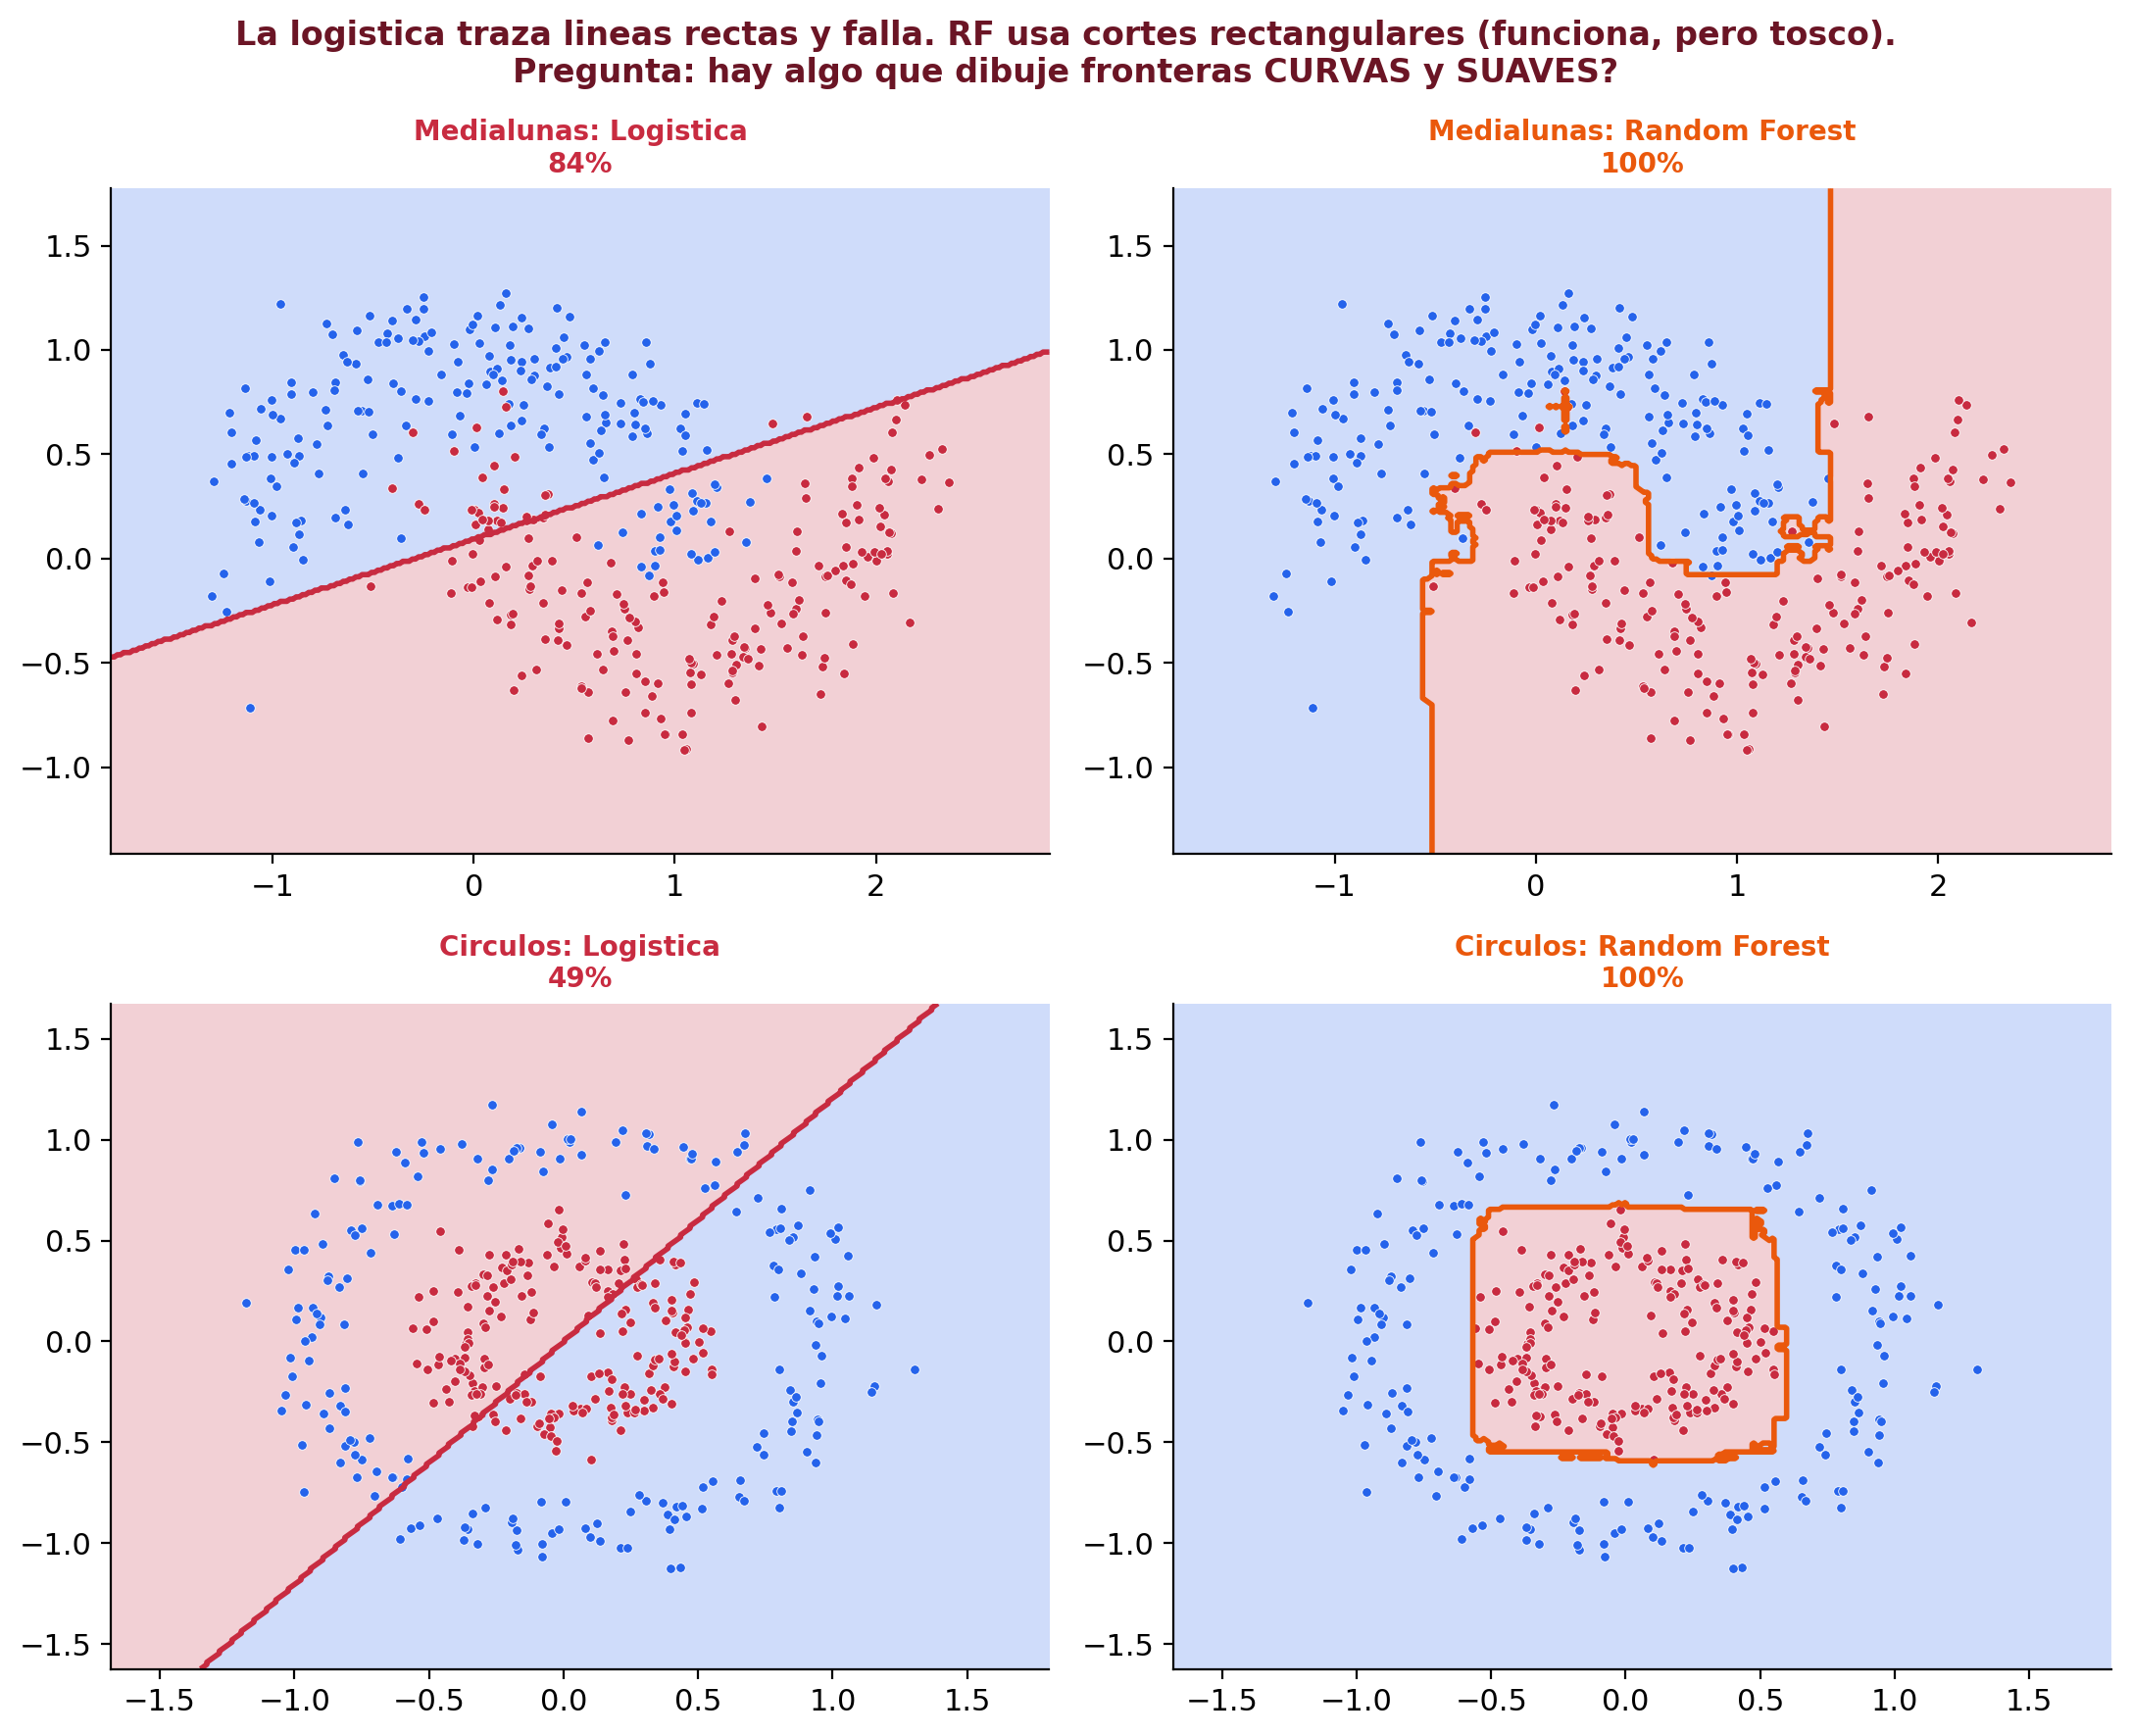
\includegraphics[width=0.88\textwidth]{fig_problema.png}
  \end{center}

  \vspace{-2pt}
  {\scriptsize\color{textMuted}
    \faLightbulb\hspace{4pt} \textbf{Fila 1:} medialunas.
    \textbf{Fila 2:} c\'irculos.
    La log\'istica traza una l\'inea recta y falla.
    RF mejora pero con cortes rectangulares --- la frontera es dentada,
    no suave. Queremos algo que dibuje \textbf{curvas}.}
\end{frame}

\begin{frame}{Recuerden MNIST (Clase 22)}
  \vspace{-4pt}
  {\footnotesize\color{arcaDark}\bfseries
    El mismo problema ocurri\'o con im\'agenes:}

  \vspace{6pt}
  {\footnotesize
  \begin{itemize}\setlength{\itemsep}{5pt}
    \item[{\color{arcaRed}\scriptsize\faArrowRight}]
      \textbf{Log\'istica en MNIST:} $\approx$ 90\%. Trata cada pixel
      como independiente --- no sabe que pixel 100 est\'a al lado de pixel 101.
    \item[{\color{codeOrange}\scriptsize\faArrowRight}]
      \textbf{Random Forest en MNIST:} $\approx$ 95\%. Mejor, pero sigue
      confundiendo 3$\leftrightarrow$8 y 9$\leftrightarrow$4.
    \item[{\color{arcaRed}\scriptsize\faArrowRight}]
      \textbf{Fashion MNIST:} log\'istica 84\%, RF 87\%.
      Con ropa el techo es a\'un m\'as bajo.
    \item[{\color{codeGreen}\scriptsize\faArrowRight}]
      \textbf{Redes neuronales en MNIST:} 99.7\%.
      En Fashion MNIST: $\approx$ 93\%.
      Hoy entenderemos \textbf{por qu\'e} y \textbf{c\'omo}.
  \end{itemize}
  }

  \vspace{4pt}
  \begin{tcolorbox}[colback=codeGreen!8, colframe=codeGreen, boxrule=0.5pt, arc=2pt,
    left=6pt, right=6pt, top=4pt, bottom=4pt]
    {\scriptsize\color{arcaDark}
    \faLightbulb\hspace{4pt}\textbf{Aplicaci\'on real:} reconocer productos
    en un anaquel, leer c\'odigos de barras da\~nados, detectar etiquetas
    mal impresas --- todo usa redes neuronales. Hoy construimos la base.}
  \end{tcolorbox}
\end{frame}

\begin{frame}{Lo que Buscamos}
  \vspace{-4pt}
  {\footnotesize\color{arcaDark}\bfseries
    Un modelo que:}

  \vspace{8pt}
  {\footnotesize
  \begin{itemize}\setlength{\itemsep}{6pt}
    \item[{\color{codeGreen}\scriptsize\faCheckCircle}]
      Pueda trazar fronteras \textbf{curvas y suaves}, no solo
      l\'ineas rectas o cortes rectangulares.
    \item[{\color{codeGreen}\scriptsize\faCheckCircle}]
      \textbf{Aprenda la forma} de los datos autom\'aticamente ---
      no necesitamos decirle si es un c\'irculo o una medialuna.
    \item[{\color{codeGreen}\scriptsize\faCheckCircle}]
      Funcione con \textbf{muchas variables} (784 pixeles, 50 features).
    \item[{\color{codeGreen}\scriptsize\faCheckCircle}]
      Use la \textbf{misma API de sklearn} que ya conocemos
      (\texttt{.fit()}, \texttt{.predict()}).
  \end{itemize}
  }

  \vspace{6pt}
  \begin{tcolorbox}[colback=codeGreen!8, colframe=codeGreen, boxrule=0.5pt, arc=2pt,
    left=6pt, right=6pt, top=4pt, bottom=4pt]
    {\scriptsize\color{arcaDark}
    \faLightbulb\hspace{4pt} Ese modelo existe: se llama \textbf{red neuronal}
    (o MLP --- Multi-Layer Perceptron). Y resulta que ya conocen
    su pieza fundamental: la \textbf{regresi\'on log\'istica}.}
  \end{tcolorbox}
\end{frame}

% =============================================================================
%  BLOQUE 2: DE LA LOG\'ISTICA A LA NEURONA
% =============================================================================
\sectionframe{De la Log\'istica a la Neurona}{Extendiendo lo que ya saben}

\begin{frame}[shrink=20]{La Log\'istica ES una Neurona}
  \vspace{-4pt}
  {\footnotesize\color{arcaDark}\bfseries
    La regresi\'on log\'istica que aprendieron en la clase 16 es,
    literalmente, \textbf{una red neuronal de una sola neurona}.
    Recuerden qu\'e hace la log\'istica:}

  \vspace{4pt}
  {\scriptsize
  \begin{enumerate}\setlength{\itemsep}{2pt}
    \item[{\color{arcaRed}\bfseries 1.}]
      Toma las variables ($x_1, x_2, \ldots$) y las multiplica por
      coeficientes ($\beta_1, \beta_2, \ldots$).
    \item[{\color{arcaRed}\bfseries 2.}]
      Suma todo + un intercepto: $z = \beta_1 x_1 + \beta_2 x_2 + \ldots + \beta_0$.
    \item[{\color{arcaRed}\bfseries 3.}]
      Pasa $z$ por la \textbf{funci\'on sigmoid} $\sigma(z) = \frac{1}{1+e^{-z}}$
      para obtener una probabilidad entre 0 y 1.
  \end{enumerate}
  }

  \vspace{2pt}
  {\scriptsize\color{arcaDark}
    \faKey\hspace{4pt} Esos 3 pasos son \textbf{exactamente} lo que
    hace una neurona artificial. Solo cambia la nomenclatura:}

  \vspace{4pt}
  \begin{center}
  \begin{tikzpicture}[
    >=Stealth, node distance=1.2cm,
    input/.style={circle, draw=codeBlue, fill=codeBlue!15, minimum size=0.6cm,
                  font=\scriptsize\bfseries},
    neuron/.style={circle, draw=arcaRed, fill=arcaRed!15, minimum size=0.85cm,
                   font=\scriptsize\bfseries},
    output/.style={circle, draw=codeGreen, fill=codeGreen!15, minimum size=0.6cm,
                   font=\scriptsize\bfseries},
    lbl/.style={font=\tiny\color{textMuted}},
  ]
    % Logística
    \node[font=\scriptsize\bfseries\color{arcaDark}] at (-0.3, 1.7) {LOG\'ISTICA};
    \node[input] (x1) at (0, 0.8) {$x_1$};
    \node[input] (x2) at (0, 0) {$x_2$};
    \node[input] (x3) at (0,-0.8) {$x_3$};
    \node[neuron] (n1) at (2.2, 0) {$\sigma(z)$};
    \node[output] (o1) at (3.8, 0) {$\hat{y}$};
    \draw[->, thick, codeBlue] (x1) -- node[above, lbl]{$\beta_1$} (n1);
    \draw[->, thick, codeBlue] (x2) -- node[above, lbl]{$\beta_2$} (n1);
    \draw[->, thick, codeBlue] (x3) -- node[below, lbl]{$\beta_3$} (n1);
    \draw[->, thick, codeGreen] (n1) -- (o1);

    % =
    \node[font=\Large\bfseries\color{arcaDark}] at (5.2, 0) {$=$};

    % Neurona
    \node[font=\scriptsize\bfseries\color{arcaDark}] at (8, 1.7) {NEURONA};
    \node[input] (a1) at (6.5, 0.8) {$x_1$};
    \node[input] (a2) at (6.5, 0) {$x_2$};
    \node[input] (a3) at (6.5,-0.8) {$x_3$};
    \node[neuron] (n2) at (8.7, 0) {$f(z)$};
    \node[output] (o2) at (10.3, 0) {$a$};
    \draw[->, thick, arcaRed] (a1) -- node[above, lbl]{$w_1$} (n2);
    \draw[->, thick, arcaRed] (a2) -- node[above, lbl]{$w_2$} (n2);
    \draw[->, thick, arcaRed] (a3) -- node[below, lbl]{$w_3$} (n2);
    \draw[->, thick, codeGreen] (n2) -- (o2);
  \end{tikzpicture}
  \end{center}

  \vspace{2pt}
  {\scriptsize
  \begin{tabular}{@{}lll@{}}
    \toprule
    \textbf{Log\'istica} & \textbf{Neurona} & \textbf{Significado} \\
    \midrule
    Coeficientes $\beta$ & Pesos $w$ & Cu\'anto influye cada variable \\
    Intercept $\beta_0$ & Bias $b$ & Desplaza la frontera de decisi\'on \\
    Sigmoid $\sigma$ & Activaci\'on $f$ & Transforma la suma en una salida \\
    \bottomrule
  \end{tabular}
  }
\end{frame}

\begin{frame}{Entonces ?`Qu\'e Cambia?}
  \vspace{-4pt}
  {\footnotesize\color{arcaDark}\bfseries
    Si la log\'istica ya es una neurona, ?`qu\'e hace distinta a una
    \textbf{red} neuronal?}

  \vspace{8pt}
  {\footnotesize
  \begin{itemize}\setlength{\itemsep}{6pt}
    \item[{\color{arcaRed}\scriptsize\faArrowRight}]
      \textbf{La log\'istica} = \textbf{1 neurona}. Solo puede
      trazar una l\'inea recta. Los pesos controlan la posici\'on
      y orientaci\'on de esa l\'inea, nada m\'as.
    \item[{\color{codeGreen}\scriptsize\faArrowRight}]
      \textbf{Una red neuronal} = \textbf{muchas neuronas conectadas
      en capas}. Cada neurona traza su propia l\'inea. La siguiente
      capa \textbf{combina} esas l\'ineas --- y la combinaci\'on
      puede ser una curva.
    \item[{\color{codeGreen}\scriptsize\faArrowRight}]
      Adem\'as, en las capas internas se puede usar una funci\'on
      de activaci\'on distinta a sigmoid (como \textbf{ReLU} o
      \textbf{Tanh}). Lo importante es que sea \textbf{no lineal}
      --- sin eso, agregar capas no agrega nada.
  \end{itemize}
  }

  \vspace{4pt}
  \begin{tcolorbox}[colback=arcaGray, colframe=arcaRed, boxrule=0.5pt, arc=2pt,
    left=6pt, right=6pt, top=4pt, bottom=4pt]
    {\scriptsize\color{arcaDark}
    \faKey\hspace{4pt}\textbf{No es un concepto nuevo.} Es el mismo
    concepto de la log\'istica, repetido muchas veces y conectado
    en capas. La potencia viene de la \textbf{composici\'on}.}
  \end{tcolorbox}
\end{frame}

\begin{frame}[shrink=18]{Visual: 1 Neurona Falla en Todo}
  \vspace{-4pt}
  \begin{center}
    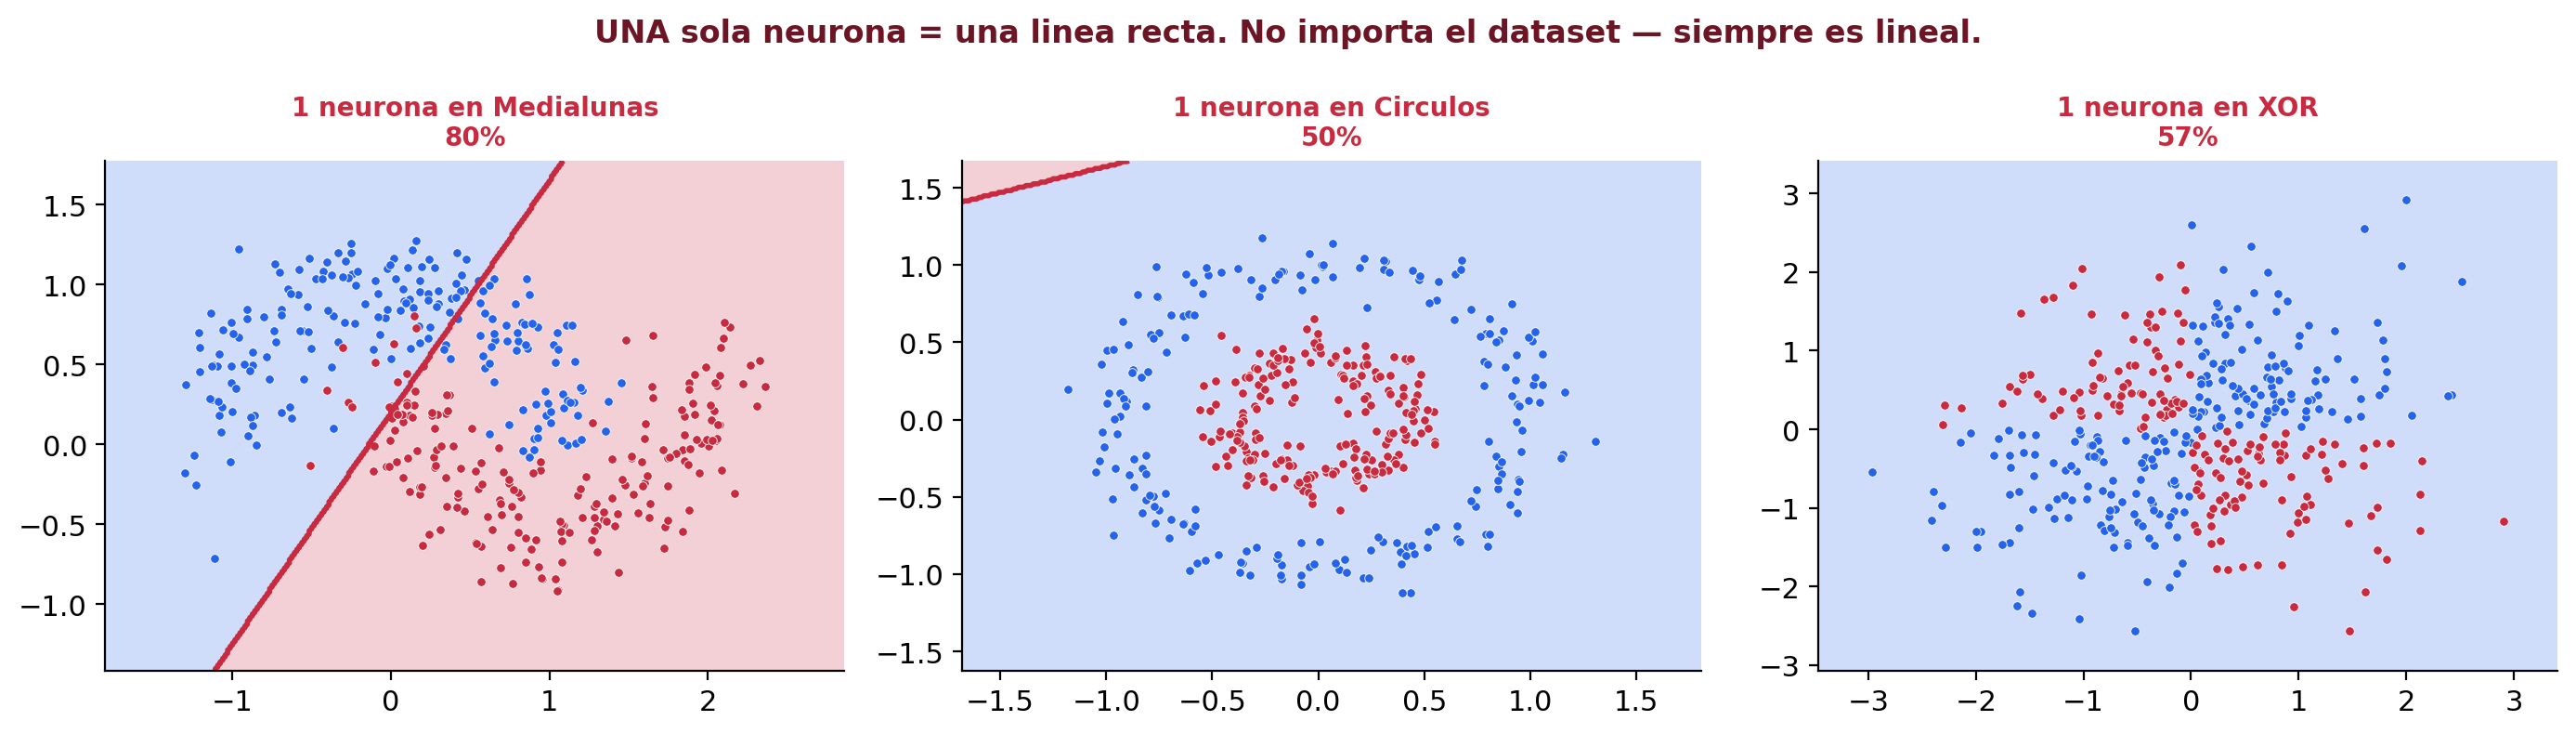
\includegraphics[width=0.88\textwidth]{fig_1neurona.png}
  \end{center}

  \vspace{-2pt}
  {\scriptsize\color{textMuted}
    \faLightbulb\hspace{4pt} Una sola neurona en medialunas (80\%),
    c\'irculos (50\%), XOR (57\%). En c\'irculos es literalmente
    azar --- la l\'inea recta no puede hacer nada.
    \textbf{Necesitamos m\'as neuronas.}}
\end{frame}

\begin{frame}{?`Por Qu\'e Se Llama ``Neurona''? --- La Inspiraci\'on Biol\'ogica}
  \vspace{-4pt}
  {\footnotesize\color{arcaDark}\bfseries
    En 1943, McCulloch y Pitts propusieron un modelo matem\'atico
    inspirado en c\'omo funcionan las neuronas del cerebro:}

  \vspace{6pt}
  {\scriptsize
  \begin{tabular}{@{}p{2.5cm}p{4.5cm}p{5cm}@{}}
    \toprule
    \textbf{Biol\'ogica} & \textbf{Funci\'on} & \textbf{Artificial} \\
    \midrule
    \textbf{Dendritas} & Reciben se\~nales de otras neuronas. & \textbf{Inputs} ($x_1, x_2, \ldots$): los datos de entrada. \\
    \textbf{Sinapsis} & Fortaleza de la conexi\'on. Se refuerza o debilita con el aprendizaje. & \textbf{Pesos} ($w_1, w_2, \ldots$): n\'umeros que se ajustan durante el entrenamiento. \\
    \textbf{Soma (cuerpo)} & Integra las se\~nales. Si superan un umbral, la neurona se activa (``dispara''). & \textbf{Suma ponderada + activaci\'on}: $z = \sum w_i x_i + b$, luego $f(z)$. \\
    \textbf{Ax\'on} & Transmite la se\~nal de salida a las siguientes neuronas. & \textbf{Output}: un n\'umero que se env\'ia a la siguiente capa. \\
    \bottomrule
  \end{tabular}
  }

  \vspace{6pt}
  {\scriptsize\color{textMuted}
    \faLightbulb\hspace{4pt} No es una r\'eplica exacta del cerebro ---
    es una \textbf{simplificaci\'on matem\'atica} que captura la idea
    esencial: recibir, integrar, decidir, transmitir.}
\end{frame}

\begin{frame}{Los Pesos: Qu\'e Inputs Importan M\'as}
  \vspace{-4pt}
  {\footnotesize\color{arcaDark}\bfseries
    Cada peso $w_i$ determina cu\'anto influye el input $x_i$
    en la decisi\'on de la neurona:}

  \vspace{6pt}
  {\footnotesize
  \begin{itemize}\setlength{\itemsep}{5pt}
    \item[{\color{arcaRed}\scriptsize\faArrowRight}]
      \textbf{Peso grande positivo} ($w = 2.5$): ese input
      influye \textbf{mucho} y en la misma direcci\'on.
      Si el input sube, el output sube.
    \item[{\color{codeBlue}\scriptsize\faArrowRight}]
      \textbf{Peso grande negativo} ($w = -1.8$): influye
      \textbf{mucho} pero al rev\'es. Si el input sube, el output baja.
    \item[{\color{textMuted}\scriptsize\faArrowRight}]
      \textbf{Peso cercano a cero} ($w = 0.01$): ese input
      casi \textbf{no importa} para esta neurona.
    \item[{\color{codeGreen}\scriptsize\faArrowRight}]
      El \textbf{bias} $b$ desplaza la frontera de decisi\'on.
      Es el intercepto $\beta_0$ de la log\'istica.
  \end{itemize}
  }

  \vspace{4pt}
  {\scriptsize\color{textMuted}
    \faLightbulb\hspace{4pt} Al inicio, los pesos son \textbf{aleatorios}
    (la neurona no sabe nada). Durante el entrenamiento, se ajustan
    para minimizar el error. Eso es ``aprender''.}
\end{frame}

\begin{frame}{?`Qu\'e Es la ``Activaci\'on'' y Por Qu\'e Importa?}
  \vspace{-4pt}
  {\footnotesize\color{arcaDark}\bfseries
    La log\'istica usa sigmoid para convertir la suma $z$ en una
    probabilidad. Esa transformaci\'on se llama \textbf{funci\'on de
    activaci\'on}. ?`Por qu\'e no usar siempre sigmoid?}

  \vspace{6pt}
  {\footnotesize
  \begin{itemize}\setlength{\itemsep}{5pt}
    \item[{\color{arcaRed}\scriptsize\faArrowRight}]
      Sigmoid funciona bien para la \textbf{salida} (queremos una
      probabilidad 0--1). Pero en las \textbf{capas internas} de una
      red tiene un problema: el gradiente se vuelve muy peque\~no
      y la red aprende lent\'isimo.
    \item[{\color{codeGreen}\scriptsize\faArrowRight}]
      En las capas internas usamos \textbf{ReLU} $f(z) = \max(0, z)$:
      si $z > 0$, lo deja pasar. Si $z \leq 0$, lo pone en cero.
      Mucho m\'as r\'apida de calcular y sin el problema del gradiente.
    \item[{\color{codePurple}\scriptsize\faArrowRight}]
      Para la salida con \textbf{m\'ultiples clases} (d\'igitos 0--9,
      vocales A/E/I/O/U): \textbf{softmax}, que convierte $K$ valores
      en $K$ probabilidades que suman 1.
  \end{itemize}
  }

  \vspace{4pt}
  \begin{tcolorbox}[colback=arcaGray, colframe=arcaRed, boxrule=0.5pt, arc=2pt,
    left=6pt, right=6pt, top=4pt, bottom=4pt]
    {\scriptsize\color{arcaDark}
    \faKey\hspace{4pt}\textbf{Regla simple:} \textbf{ReLU} en capas
    ocultas, \textbf{sigmoid} en salida binaria, \textbf{softmax}
    en salida multiclase. sklearn configura todo con
    \texttt{activation="relu"} (default).}
  \end{tcolorbox}
\end{frame}

\begin{frame}[shrink=15]{Las Activaciones --- Visual}
  \vspace{-4pt}
  \begin{center}
    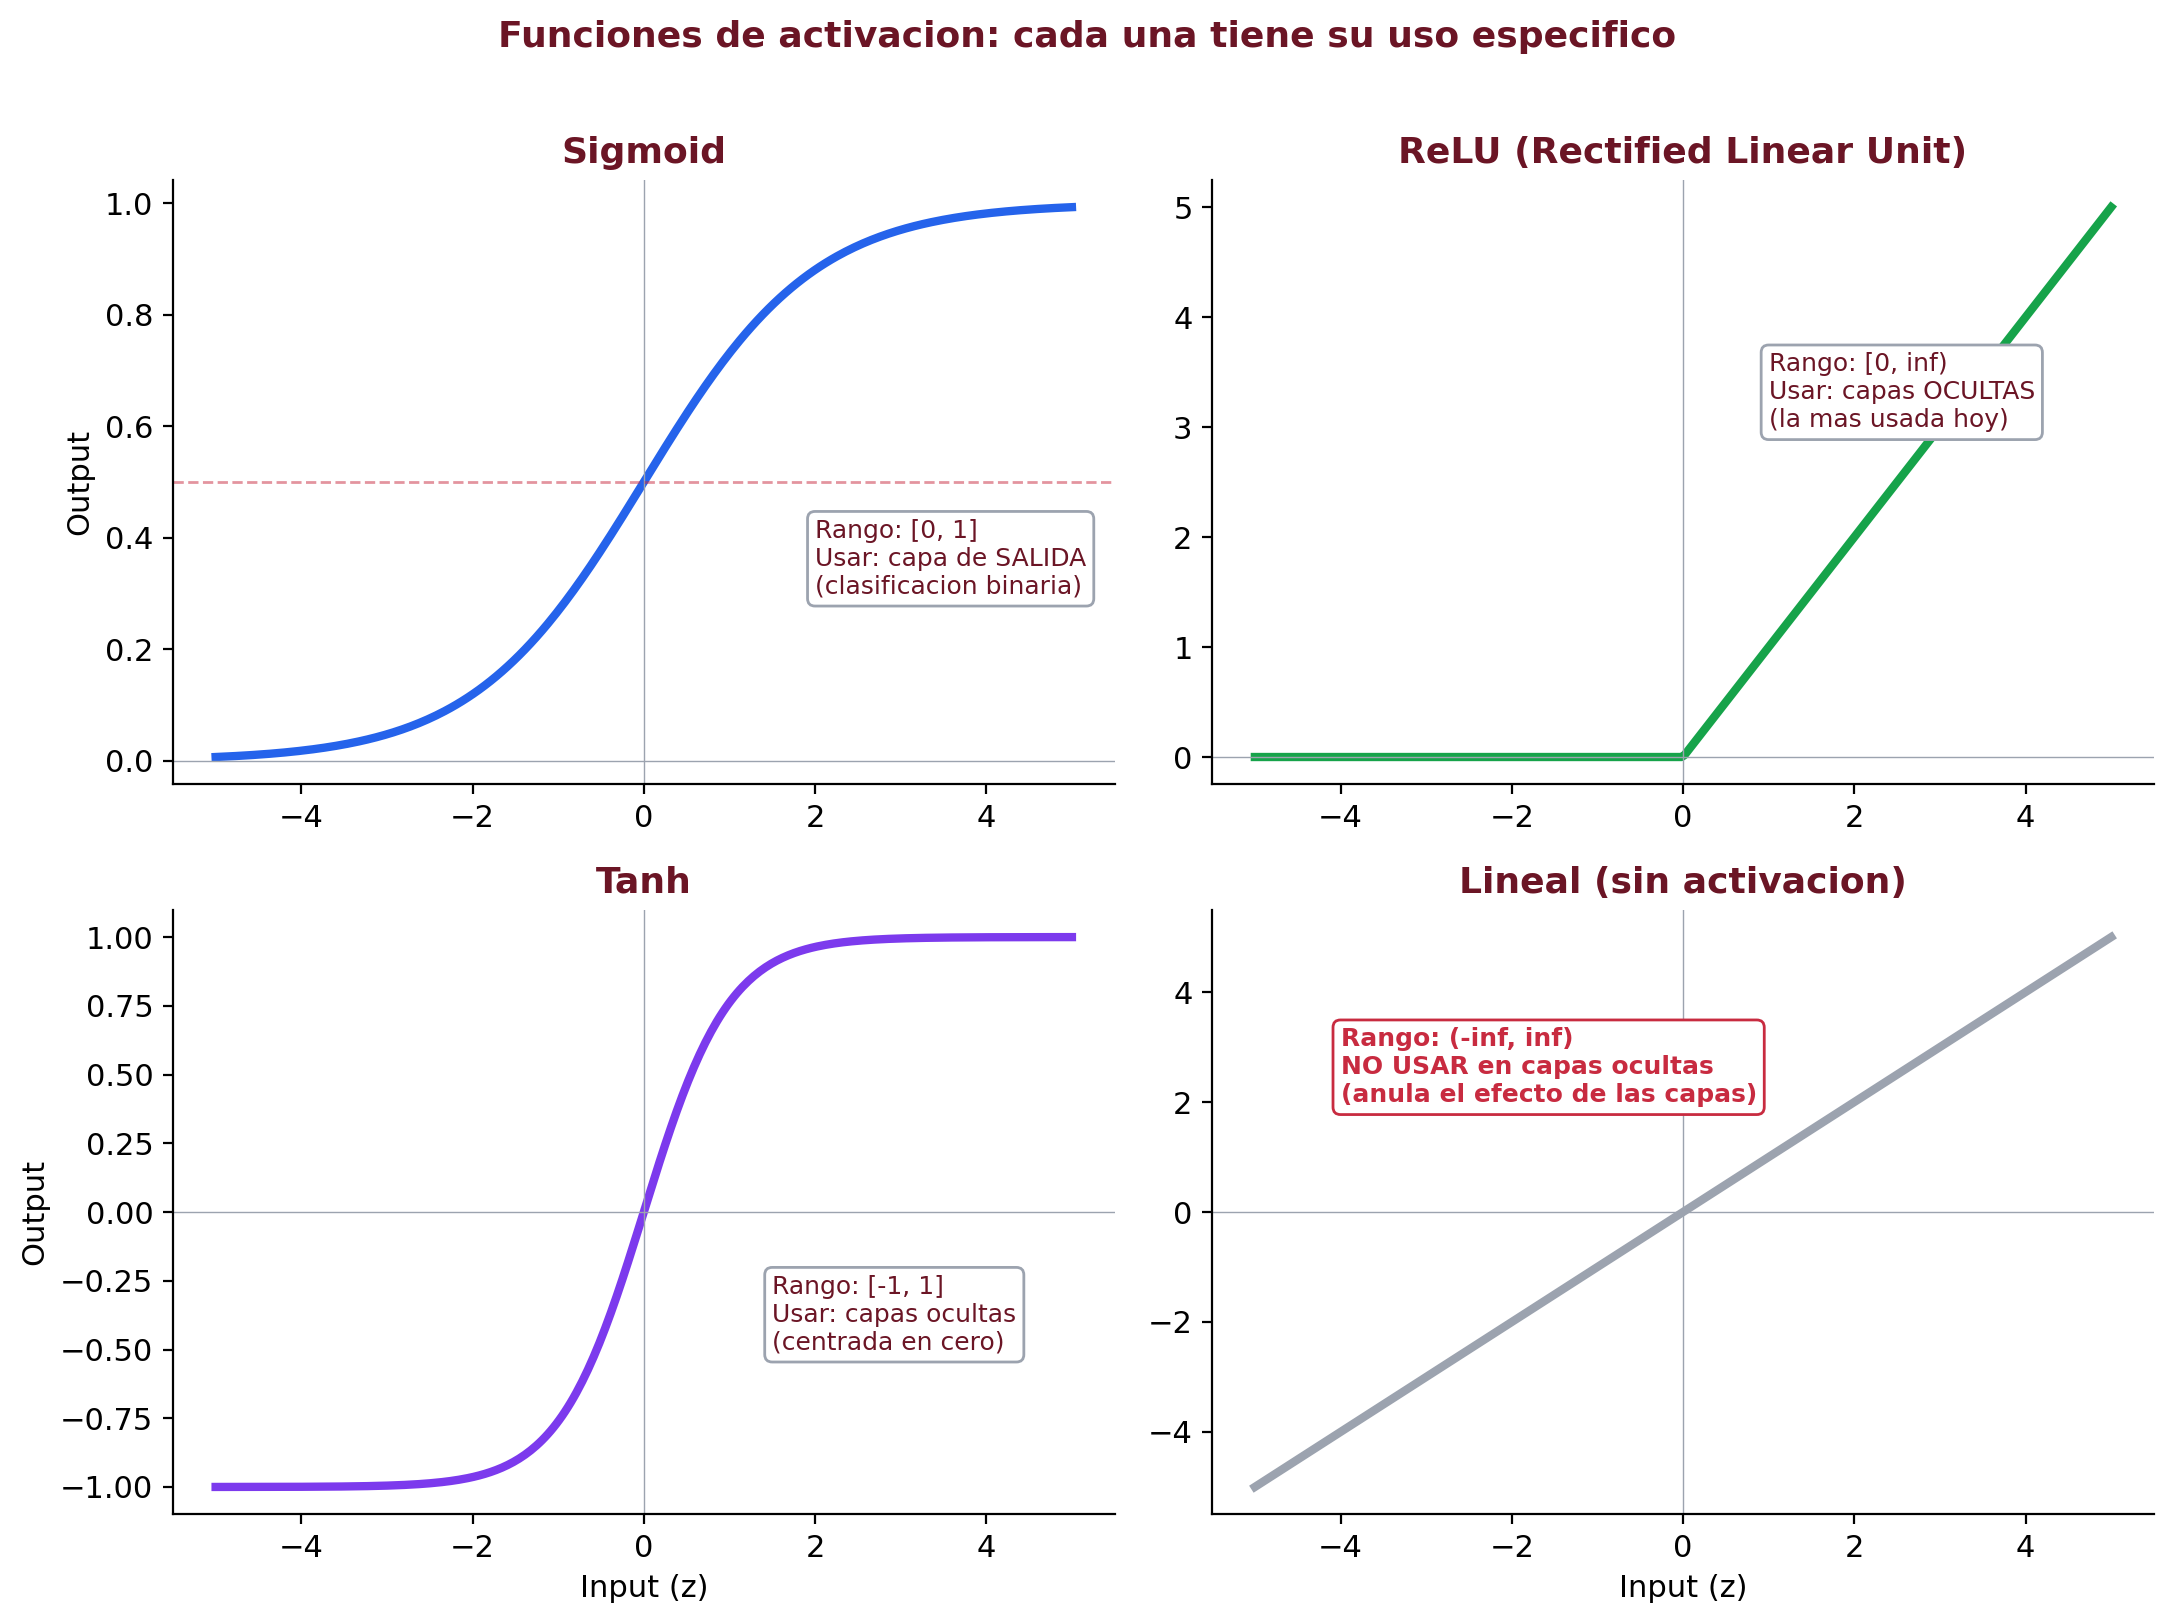
\includegraphics[width=0.88\textwidth]{fig_activaciones.png}
  \end{center}

  \vspace{-2pt}
  {\scriptsize\color{textMuted}
    \faLightbulb\hspace{4pt} Cada activaci\'on tiene su lugar.
    \textbf{ReLU:} capas ocultas (la est\'andar hoy).
    \textbf{Sigmoid:} salida binaria (s\'i/no).
    \textbf{Lineal:} \textbf{nunca} en capas ocultas --- anula
    el efecto de agregar capas (sin activaci\'on, 100 capas
    equivalen a 1 sola capa).}
\end{frame}

% =============================================================================
%  BLOQUE 3: CONECTAR NEURONAS — QU\'E VIAJA, QU\'E DETECTA CADA CAPA
% =============================================================================
\sectionframe{Conectar Neuronas}{Qu\'e viaja por las conexiones y qu\'e detecta cada capa}

\begin{frame}{?`Qu\'e Viaja por una Conexi\'on?}
  \vspace{-4pt}
  {\footnotesize\color{arcaDark}\bfseries
    Cada l\'inea que conecta dos neuronas es un ``cable con un
    multiplicador'':}

  \vspace{6pt}
  \begin{center}
  \begin{tikzpicture}[
    >=Stealth,
    neuron/.style={circle, draw=arcaRed, fill=arcaRed!15, minimum size=0.9cm,
                   font=\scriptsize\bfseries},
    lbl/.style={font=\scriptsize\color{textDark}},
    wlbl/.style={font=\scriptsize\bfseries\color{codeBlue}},
  ]
    \node[neuron, fill=codeBlue!15, draw=codeBlue] (a) at (0, 1.5) {$a_1$};
    \node[neuron, fill=codeBlue!15, draw=codeBlue] (b) at (0, 0)   {$a_2$};
    \node[neuron, fill=codeBlue!15, draw=codeBlue] (c) at (0,-1.5) {$a_3$};
    \node[neuron] (d) at (5, 0) {$\Sigma \to f$};

    \draw[->, thick, arcaRed!70] (a) -- node[above, wlbl]{$w_1 = 0.5$} (d);
    \draw[->, thick, arcaRed!70] (b) -- node[above, wlbl]{$w_2 = -0.3$} (d);
    \draw[->, thick, arcaRed!70] (c) -- node[below, wlbl]{$w_3 = 0.7$} (d);

    \node[lbl, left=4pt] at (a.west) {output = 0.8};
    \node[lbl, left=4pt] at (b.west) {output = 0.2};
    \node[lbl, left=4pt] at (c.west) {output = 0.9};

    \node[lbl, right=6pt, text width=5cm] at (d.east)
      {$z = 0.8 \times 0.5 + 0.2 \times (-0.3) + 0.9 \times 0.7$\\
       $z = 0.40 - 0.06 + 0.63 = 0.97$\\
       $\text{ReLU}(0.97) = 0.97$ \checkmark};
  \end{tikzpicture}
  \end{center}

  \vspace{4pt}
  {\scriptsize\color{arcaDark}
  \begin{itemize}\setlength{\itemsep}{3pt}
    \item[{\color{arcaRed}\scriptsize\faArrowRight}]
      Por cada conexi\'on viaja \textbf{un n\'umero}: el output de la
      neurona anterior.
    \item[{\color{arcaRed}\scriptsize\faArrowRight}]
      El \textbf{peso} multiplica esa se\~nal: la amplifica, la
      aten\'ua, o la invierte.
    \item[{\color{codeGreen}\scriptsize\faArrowRight}]
      La neurona receptora \textbf{suma todas} las se\~nales
      ponderadas y decide si se activa.
  \end{itemize}
  }
\end{frame}

\begin{frame}{?`Por Qu\'e Muchas Entradas Son \'Utiles?}
  \vspace{-4pt}
  {\footnotesize\color{arcaDark}\bfseries
    Cada neurona de la capa oculta aprende a detectar un
    \textbf{patr\'on diferente} en los datos de entrada:}

  \vspace{6pt}
  {\footnotesize
  \begin{itemize}\setlength{\itemsep}{5pt}
    \item[{\color{arcaRed}\scriptsize\faArrowRight}]
      \textbf{Neurona 1:} detecta si hay un borde horizontal en
      la zona superior de la imagen.
    \item[{\color{arcaRed}\scriptsize\faArrowRight}]
      \textbf{Neurona 2:} detecta si hay una curva en la zona central.
    \item[{\color{arcaRed}\scriptsize\faArrowRight}]
      \textbf{Neurona 3:} detecta si la parte inferior est\'a vac\'ia.
    \item[{\color{codeGreen}\scriptsize\faArrowRight}]
      La neurona de la \textbf{siguiente capa} combina: ``borde arriba
      + curva al centro + vac\'io abajo = probablemente un \textbf{7}''.
  \end{itemize}
  }

  \vspace{4pt}
  \begin{tcolorbox}[colback=arcaGray, colframe=arcaRed, boxrule=0.5pt, arc=2pt,
    left=6pt, right=6pt, top=4pt, bottom=4pt]
    {\scriptsize\color{arcaDark}
    \faKey\hspace{4pt}\textbf{Ninguna neurona sola sabe que es un 7.}
    Pero al combinar las ``opiniones'' de muchas neuronas, cada una
    mirando un aspecto diferente, la red s\'i puede saberlo.
    Es como un equipo: un analista ve ventas, otro log\'istica, otro
    marketing --- juntos entienden m\'as que cualquiera solo.}
  \end{tcolorbox}
\end{frame}

\begin{frame}{Fully Connected: La Estructura del MLP}
  \vspace{-4pt}
  {\footnotesize\color{arcaDark}\bfseries
    En un MLP (Multi-Layer Perceptron), cada neurona de una capa
    est\'a conectada a \textbf{todas} las neuronas de la siguiente.
    Por eso se llama ``fully connected'' o ``densa''.}

  \vspace{6pt}
  {\footnotesize
  \begin{itemize}\setlength{\itemsep}{4pt}
    \item[{\color{codeBlue}\scriptsize\faArrowRight}]
      \textbf{Capa de entrada:} una ``neurona'' por variable.
      No calcula nada, solo pasa los datos.
    \item[{\color{arcaRed}\scriptsize\faArrowRight}]
      \textbf{Capas ocultas:} donde la red aprende patrones.
      Cu\'antas capas y neuronas por capa lo elegimos nosotros.
    \item[{\color{codeGreen}\scriptsize\faArrowRight}]
      \textbf{Capa de salida:} una neurona por clase.
      Usa sigmoid (binario) o softmax (multiclase).
  \end{itemize}
  }

  \vspace{4pt}
  \begin{center}
    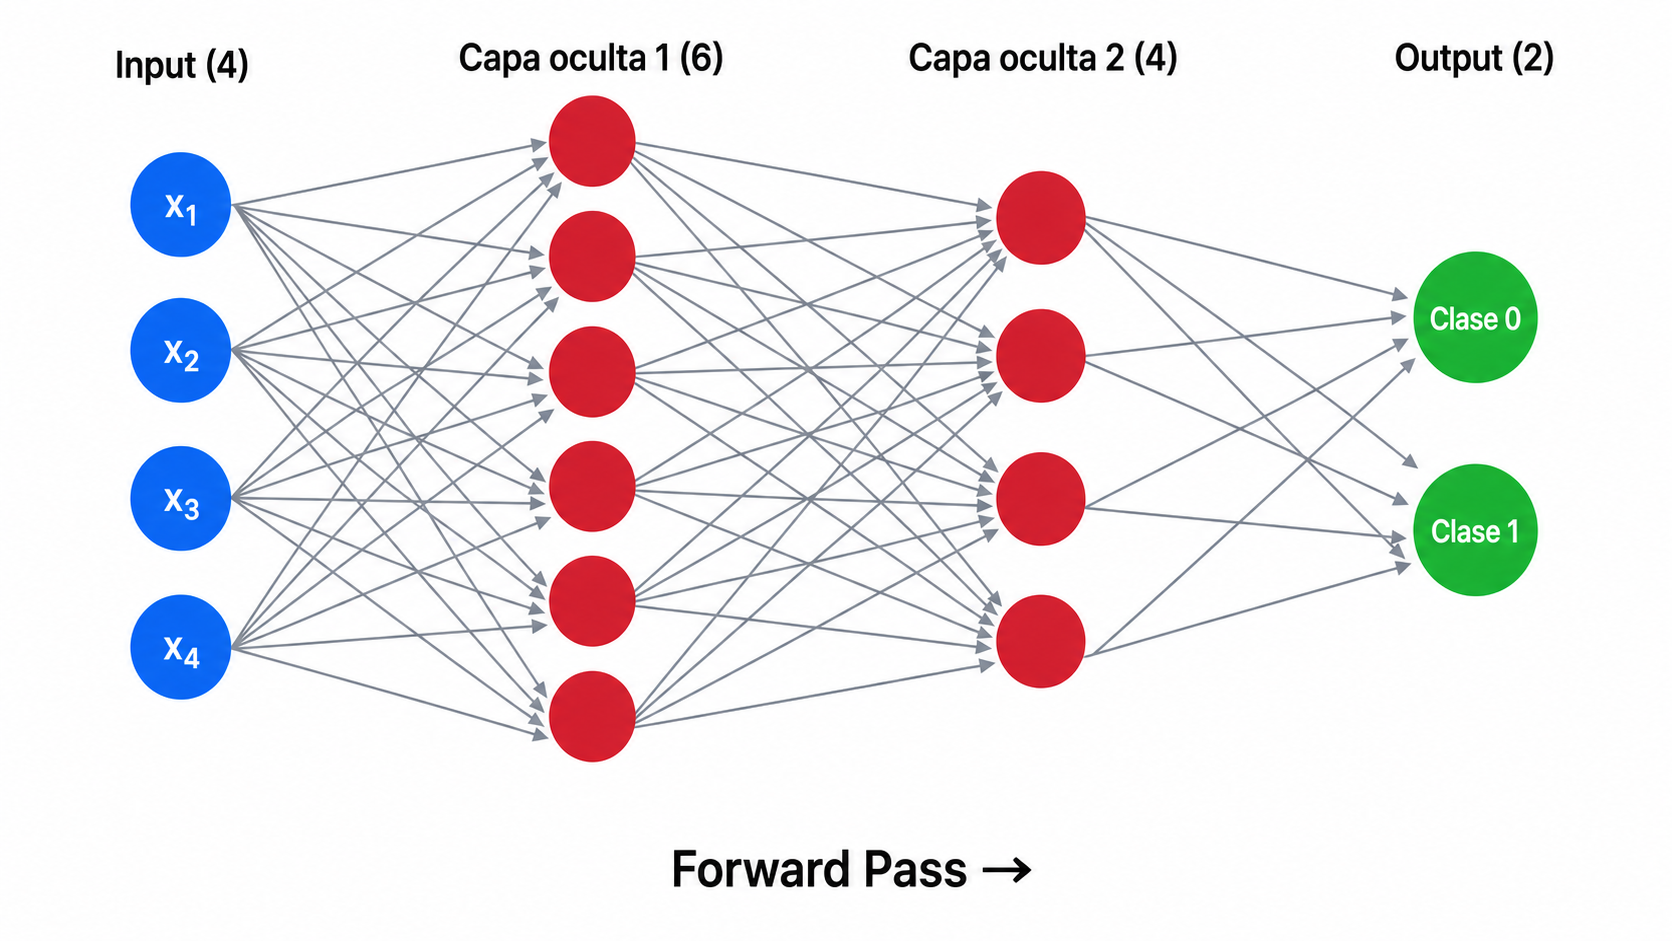
\includegraphics[width=0.5\textwidth]{neurona.png}
  \end{center}
\end{frame}

\begin{frame}{Qu\'e Detecta Cada Nivel}
  \vspace{-4pt}
  {\footnotesize\color{arcaDark}\bfseries
    Las capas forman una jerarqu\'ia de patrones, de lo simple
    a lo complejo:}

  \vspace{6pt}
  {\footnotesize
  \begin{itemize}\setlength{\itemsep}{5pt}
    \item[{\color{codeBlue}\scriptsize\faArrowRight}]
      \textbf{Primera capa oculta:} detecta patrones \textbf{simples}
      directamente en los inputs. En im\'agenes: bordes, l\'ineas,
      gradientes. En datos tabulares: umbrales y rangos.
    \item[{\color{arcaRed}\scriptsize\faArrowRight}]
      \textbf{Segunda capa:} combina esos patrones simples en patrones
      \textbf{intermedios}. En im\'agenes: esquinas, curvas, texturas.
    \item[{\color{codeGreen}\scriptsize\faArrowRight}]
      \textbf{Tercera capa:} combina patrones intermedios en patrones
      \textbf{complejos}. En im\'agenes: partes de objetos (ojo, rueda,
      el ``lazo'' de un 8).
    \item[{\color{codePurple}\scriptsize\faArrowRight}]
      \textbf{Capas profundas:} conceptos completos (``es un gato'',
      ``es un 3''). Esta jerarqu\'ia es lo que hace poderosas a las
      redes profundas (deep learning).
  \end{itemize}
  }

  \vspace{4pt}
  {\scriptsize\color{textMuted}
    \faLightbulb\hspace{4pt} Para los problemas de este diplomado
    (datos tabulares, im\'agenes peque\~nas), 1--2 capas son suficientes.
    Deep learning (10+ capas) es para im\'agenes grandes, texto, audio.}
\end{frame}

\begin{frame}[shrink=18]{Visual: La Frontera Evoluciona con la Capacidad}
  \vspace{-4pt}
  \begin{center}
    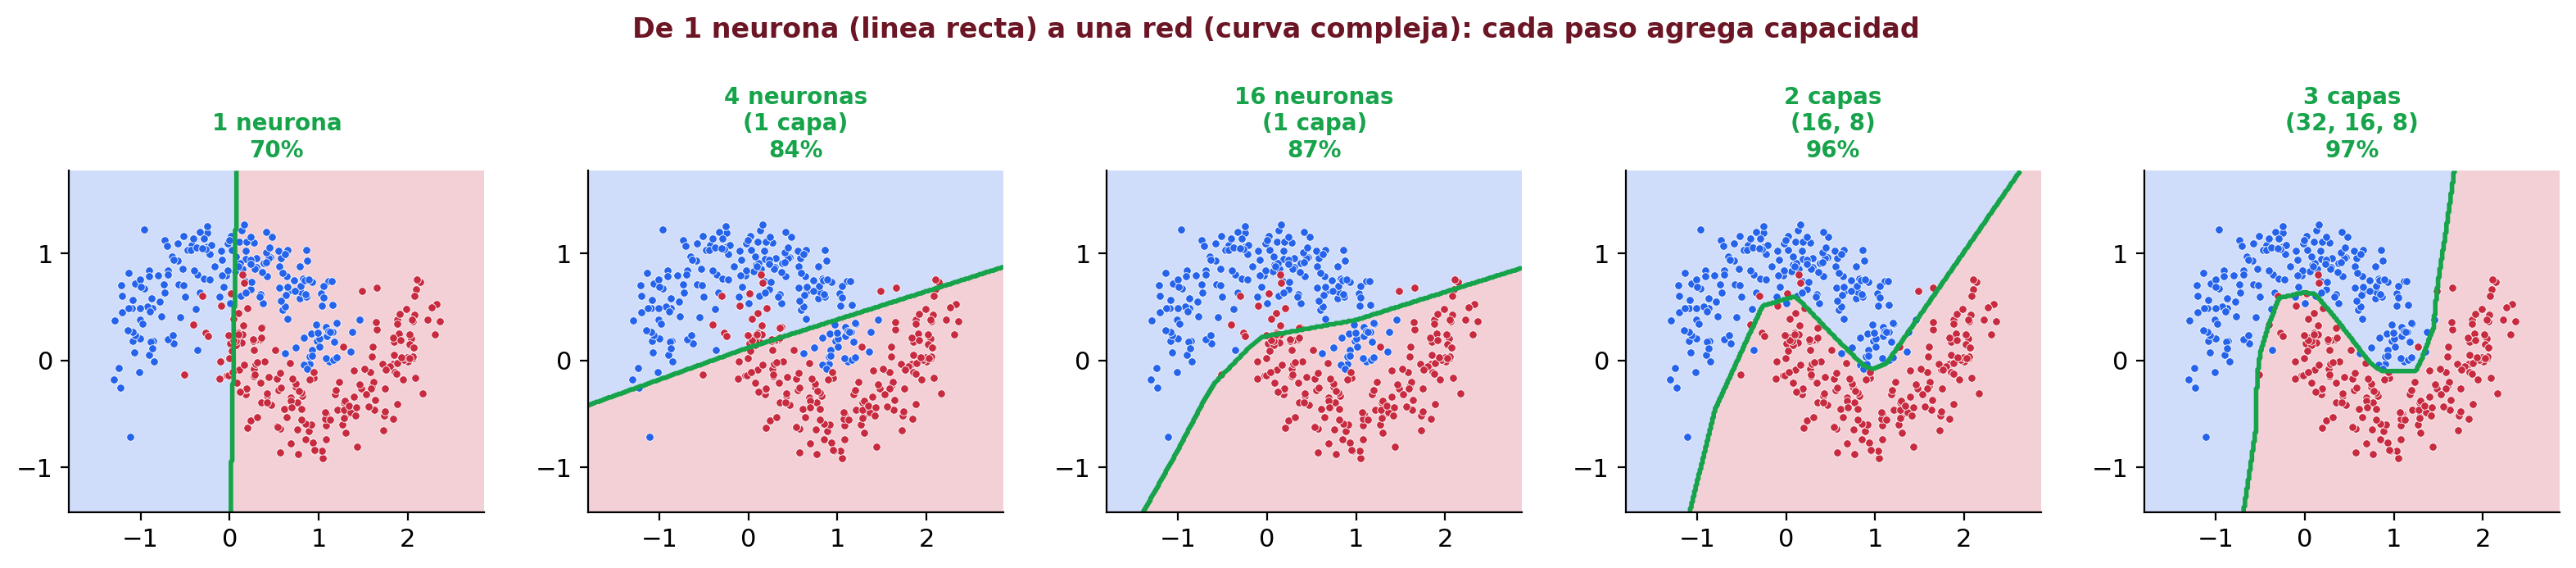
\includegraphics[width=0.95\textwidth]{fig_capas.png}
  \end{center}

  \vspace{-2pt}
  {\scriptsize\color{textMuted}
    \faLightbulb\hspace{4pt} De izquierda a derecha: \textbf{1 neurona}
    (l\'inea recta, 70\%) $\to$ \textbf{4 neuronas} (empieza a curvarse, 84\%)
    $\to$ \textbf{16 neuronas} (sigue la forma, 87\%)
    $\to$ \textbf{2 capas} (curva compleja, 96\%)
    $\to$ \textbf{3 capas} (frontera suave, 97\%).
    Cada paso agrega capacidad para formas m\'as complejas.}
\end{frame}

\begin{frame}[shrink=18]{Demostraci\'on: Con vs Sin Activaci\'on}
  \vspace{-4pt}
  \begin{center}
    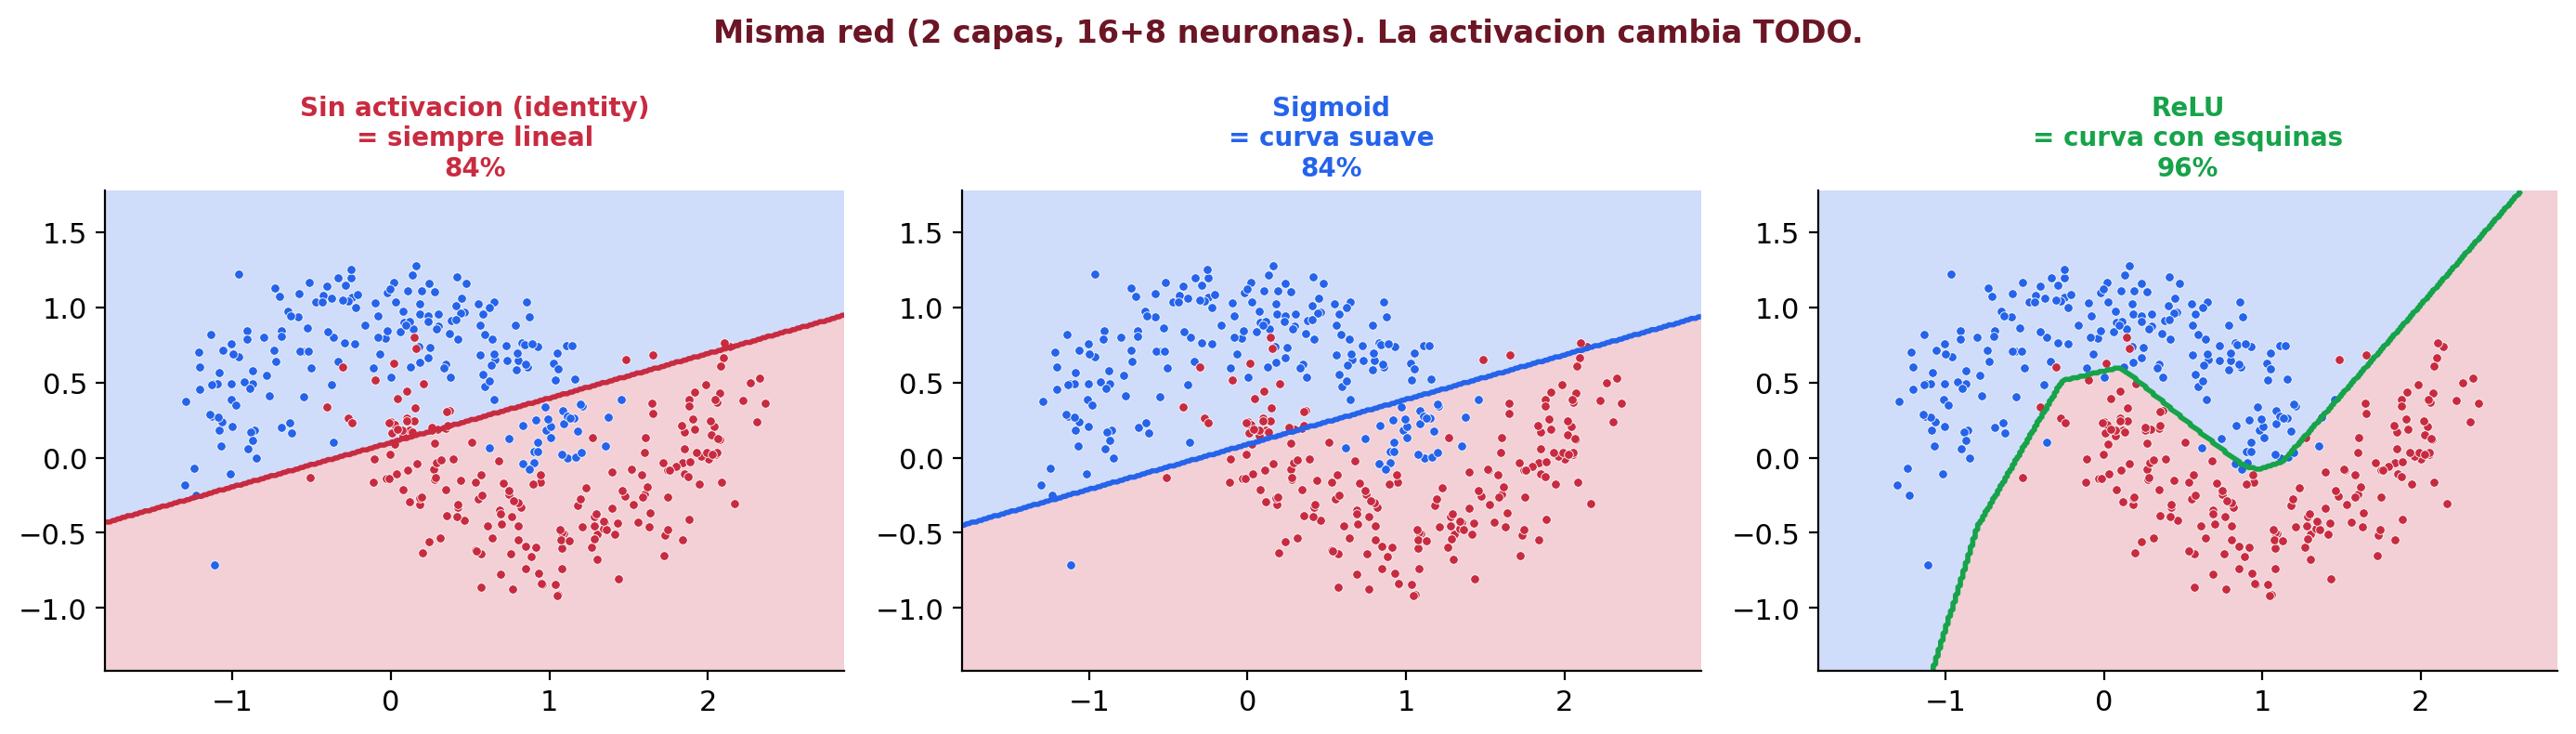
\includegraphics[width=0.88\textwidth]{fig_activacion_importa.png}
  \end{center}

  \vspace{-2pt}
  {\scriptsize\color{textMuted}
    \faLightbulb\hspace{4pt} \textbf{Misma red} (2 capas, 16+8 neuronas),
    \textbf{mismos datos.} Solo cambia la activaci\'on.
    Sin activaci\'on: l\'inea recta (84\%).
    Con sigmoid: curva suave (84\%).
    Con ReLU: curva con esquinas (96\%).
    \textbf{La activaci\'on es la diferencia entre fracaso y \'exito.}}
\end{frame}

\begin{frame}[shrink=5]{Ejercicio 1: Ver las Limitaciones con Sus Propios Ojos}
  \vspace{-4pt}
  {\footnotesize\color{arcaDark}\bfseries
    \faClock\hspace{4pt} 10 minutos --- en el notebook:}

  \vspace{6pt}
  {\footnotesize
  \begin{enumerate}\setlength{\itemsep}{4pt}
    \item[{\color{arcaRed}\bfseries 1.}]
      Generar \texttt{make\_moons(n\_samples=1000, noise=0.25)}
      y \texttt{make\_circles(n\_samples=1000, noise=0.1, factor=0.4)}.
    \item[{\color{arcaRed}\bfseries 2.}]
      Entrenar \texttt{LogisticRegression} en ambos. ?`Qu\'e accuracy da?
    \item[{\color{arcaRed}\bfseries 3.}]
      Entrenar \texttt{RandomForestClassifier(n\_estimators=100)}
      en ambos. ?`Mejora?
    \item[{\color{arcaRed}\bfseries 4.}]
      Visualizar las fronteras de decisi\'on de ambos modelos
      (\texttt{DecisionBoundaryDisplay}).
    \item[{\color{codeGreen}\bfseries 5.}]
      \textbf{Reflexi\'on:} ?`la log\'istica puede resolver c\'irculos?
      ?`RF los resuelve bien o la frontera es ``dentada''?
  \end{enumerate}
  }

  \vspace{4pt}
  {\scriptsize\color{textMuted}
    \faLightbulb\hspace{4pt} Despu\'es de este ejercicio veremos el modelo
    que s\'i puede trazar curvas suaves: el MLP.}
\end{frame}

% =============================================================================
%  BLOQUE 4: C\'OMO APRENDE LA RED (SIMPLIFICADO)
% =============================================================================
\sectionframe{C\'omo Aprende la Red}{Forward, loss, backprop, update}

\begin{frame}{El Ciclo de Aprendizaje --- 4 Pasos}
  \vspace{-4pt}
  {\footnotesize\color{arcaDark}\bfseries
    La red empieza con pesos \textbf{aleatorios}. No sabe nada.
    Aprende repitiendo este ciclo:}

  \vspace{6pt}
  {\footnotesize
  \begin{enumerate}\setlength{\itemsep}{5pt}
    \item[{\color{arcaRed}\bfseries 1.}]
      \textbf{Forward pass:} los datos entran por la izquierda,
      pasan capa por capa (multiplicar por pesos $+$ activaci\'on),
      y salen por la derecha como una predicci\'on.
      Con pesos aleatorios, la predicci\'on es basura.
    \item[{\color{arcaRed}\bfseries 2.}]
      \textbf{Calcular el loss:} comparar la predicci\'on con la
      respuesta correcta. Un n\'umero: qu\'e tan mal estuvo.
      sklearn usa \textbf{cross-entropy} (penaliza m\'as las
      predicciones confiadas y equivocadas).
    \item[{\color{codeGreen}\bfseries 3.}]
      \textbf{Backpropagation:} propagar el error \textbf{hacia atr\'as}.
      Para cada peso, calcular: ``?`cu\'anto contribuiste al error?''
      Los pesos m\'as responsables se ajustan m\'as.
    \item[{\color{codeGreen}\bfseries 4.}]
      \textbf{Actualizar pesos:} ajustar cada peso un poquito en la
      direcci\'on que reduce el error.
  \end{enumerate}
  }

  \vspace{4pt}
  {\scriptsize\color{textMuted}
    \faLightbulb\hspace{4pt} Este ciclo se repite por cada \textbf{\'epoca}
    (una pasada por todos los datos). T\'ipicamente: 50--500 \'epocas.}
\end{frame}

\begin{frame}{Backpropagation: La Cadena de Responsabilidad}
  \vspace{-4pt}
  {\footnotesize\color{arcaDark}\bfseries
    ``Backprop'' suena intimidante, pero la idea es simple:}

  \vspace{6pt}
  {\footnotesize
  \begin{itemize}\setlength{\itemsep}{5pt}
    \item[{\color{arcaRed}\scriptsize\faArrowRight}]
      La red predijo ``O'' cuando era ``A''. El loss es alto.
    \item[{\color{arcaRed}\scriptsize\faArrowRight}]
      ?`Qui\'en tuvo la culpa? La \'ultima capa us\'o los pesos
      equivocados. Pero la \'ultima capa recibi\'o inputs de la
      pen\'ultima --- quiz\'a el error viene de ah\'i.
    \item[{\color{arcaRed}\scriptsize\faArrowRight}]
      Backprop \textbf{asigna responsabilidad} a cada peso:
      ``este peso contribuy\'o 30\% al error, este 5\%, este 0.1\%\ldots''
    \item[{\color{codeGreen}\scriptsize\faArrowRight}]
      Los pesos m\'as responsables se ajustan m\'as. Los menos
      responsables, casi nada.
  \end{itemize}
  }

  \vspace{4pt}
  \begin{tcolorbox}[colback=arcaGray, colframe=arcaRed, boxrule=0.5pt, arc=2pt,
    left=6pt, right=6pt, top=4pt, bottom=4pt]
    {\scriptsize\color{arcaDark}
    \faKey\hspace{4pt} No necesitan entender las derivadas. Necesitan
    entender la idea: \textbf{cada peso recibe feedback} de cu\'anto
    contribuy\'o al error, y se ajusta proporcionalmente.}
  \end{tcolorbox}
\end{frame}

\begin{frame}{Gradient Descent: Bajar la Monta\~na}
  \vspace{-4pt}
  {\footnotesize\color{arcaDark}\bfseries
    El ajuste de pesos sigue una regla simple:}

  \vspace{6pt}
  {\footnotesize
  $$w_{\text{nuevo}} = w_{\text{viejo}} - \text{learning\_rate} \times \text{gradiente}$$
  }

  \vspace{4pt}
  {\footnotesize
  \begin{itemize}\setlength{\itemsep}{5pt}
    \item[{\color{arcaRed}\scriptsize\faArrowRight}]
      El \textbf{gradiente} dice la \textbf{direcci\'on} en la que el
      error crece m\'as r\'apido. Queremos ir en la direcci\'on
      \textbf{opuesta} (por eso el signo $-$).
    \item[{\color{arcaRed}\scriptsize\faArrowRight}]
      El \textbf{learning rate} dice qu\'e tan \textbf{grande} es
      el paso. Es un hiperpar\'ametro que elegimos nosotros.
    \item[{\color{codeGreen}\scriptsize\faArrowRight}]
      Es como bajar una monta\~na con niebla: no ves el valle,
      pero sientes la pendiente bajo tus pies y das un paso cuesta
      abajo. Repites hasta llegar al fondo.
  \end{itemize}
  }
\end{frame}

\begin{frame}[shrink=15]{Gradient Descent --- Visual}
  \vspace{-4pt}
  \begin{center}
    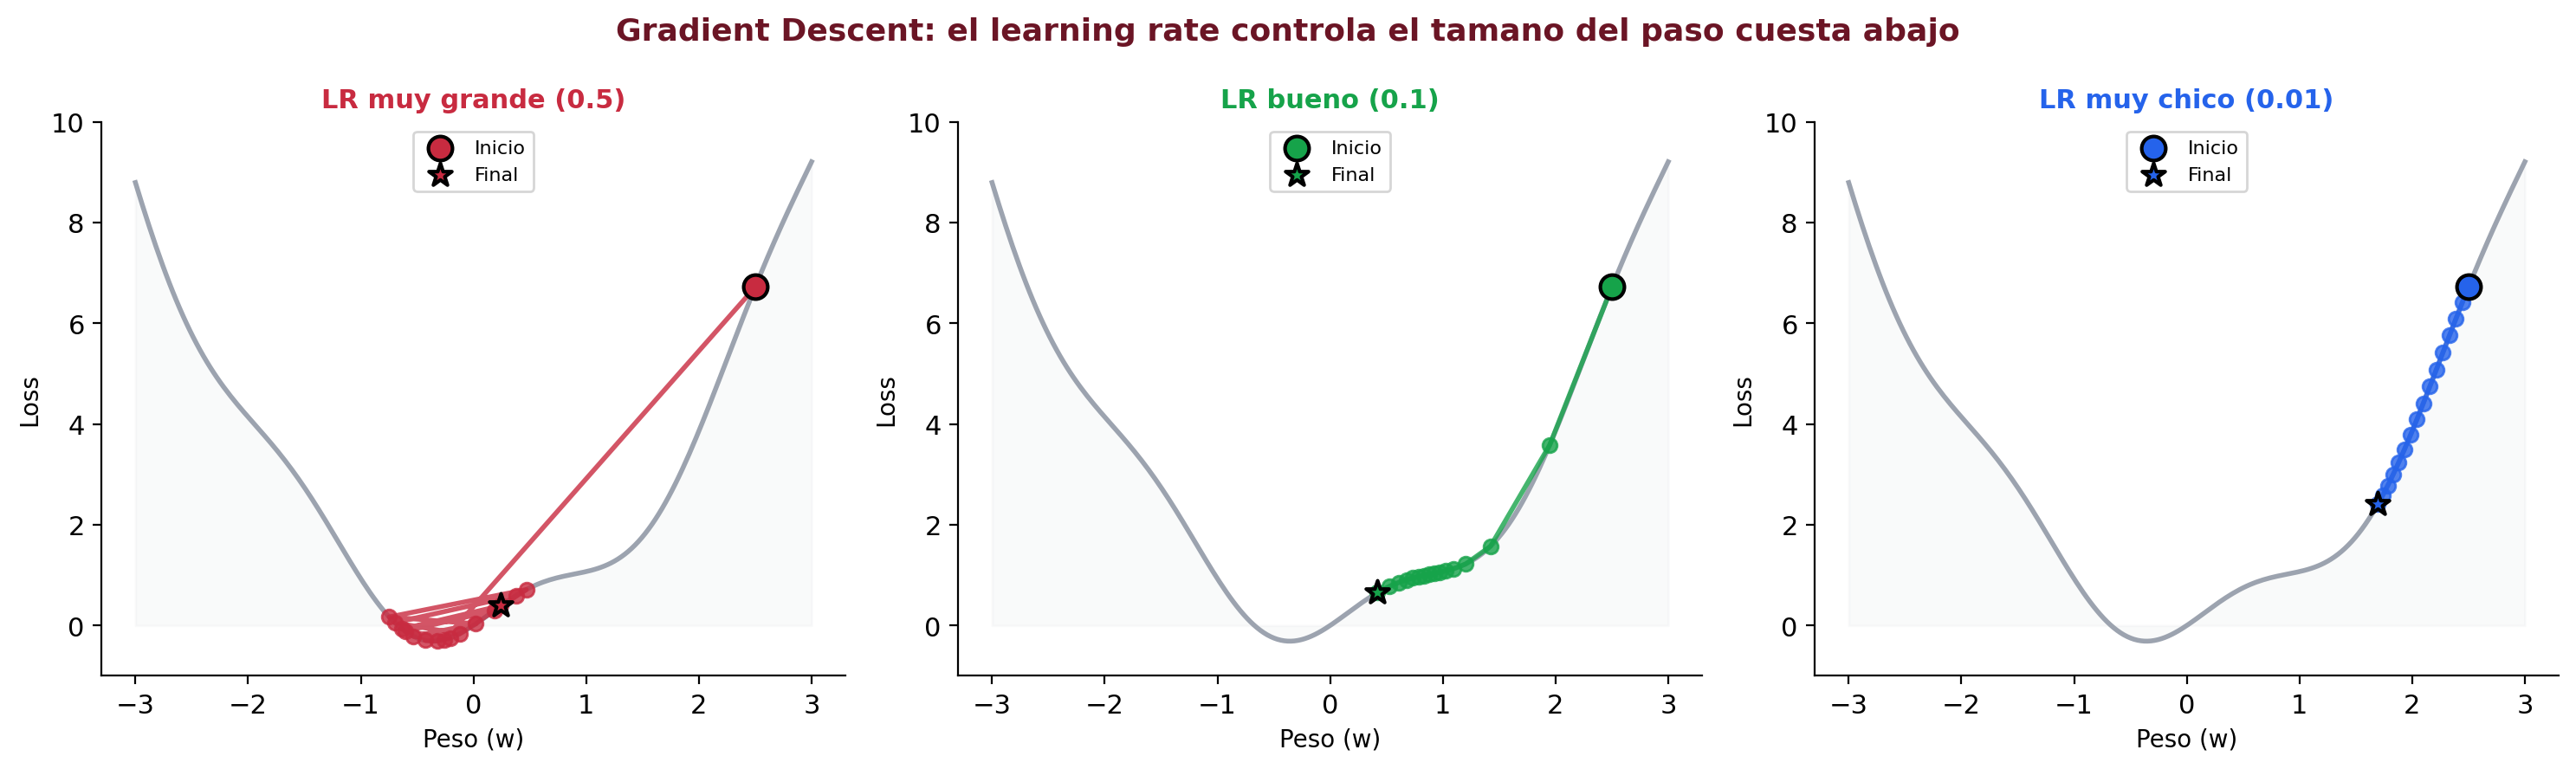
\includegraphics[width=0.95\textwidth]{fig_gradient_descent.png}
  \end{center}

  \vspace{-2pt}
  {\scriptsize\color{textMuted}
    \faLightbulb\hspace{4pt} La curva es el ``paisaje del loss'' --- queremos
    llegar al punto m\'as bajo. El c\'irculo es el inicio (pesos aleatorios),
    la estrella es donde termin\'o. \textbf{Izquierda:} pasos muy grandes
    (LR=0.5), salta de un lado a otro. \textbf{Centro:} pasos correctos
    (LR=0.1), baja r\'apido. \textbf{Derecha:} pasos muy chicos (LR=0.01),
    apenas avanza.}
\end{frame}

\begin{frame}[shrink=18]{C\'omo Leer la Curva de Loss}
  \vspace{-4pt}
  \begin{center}
    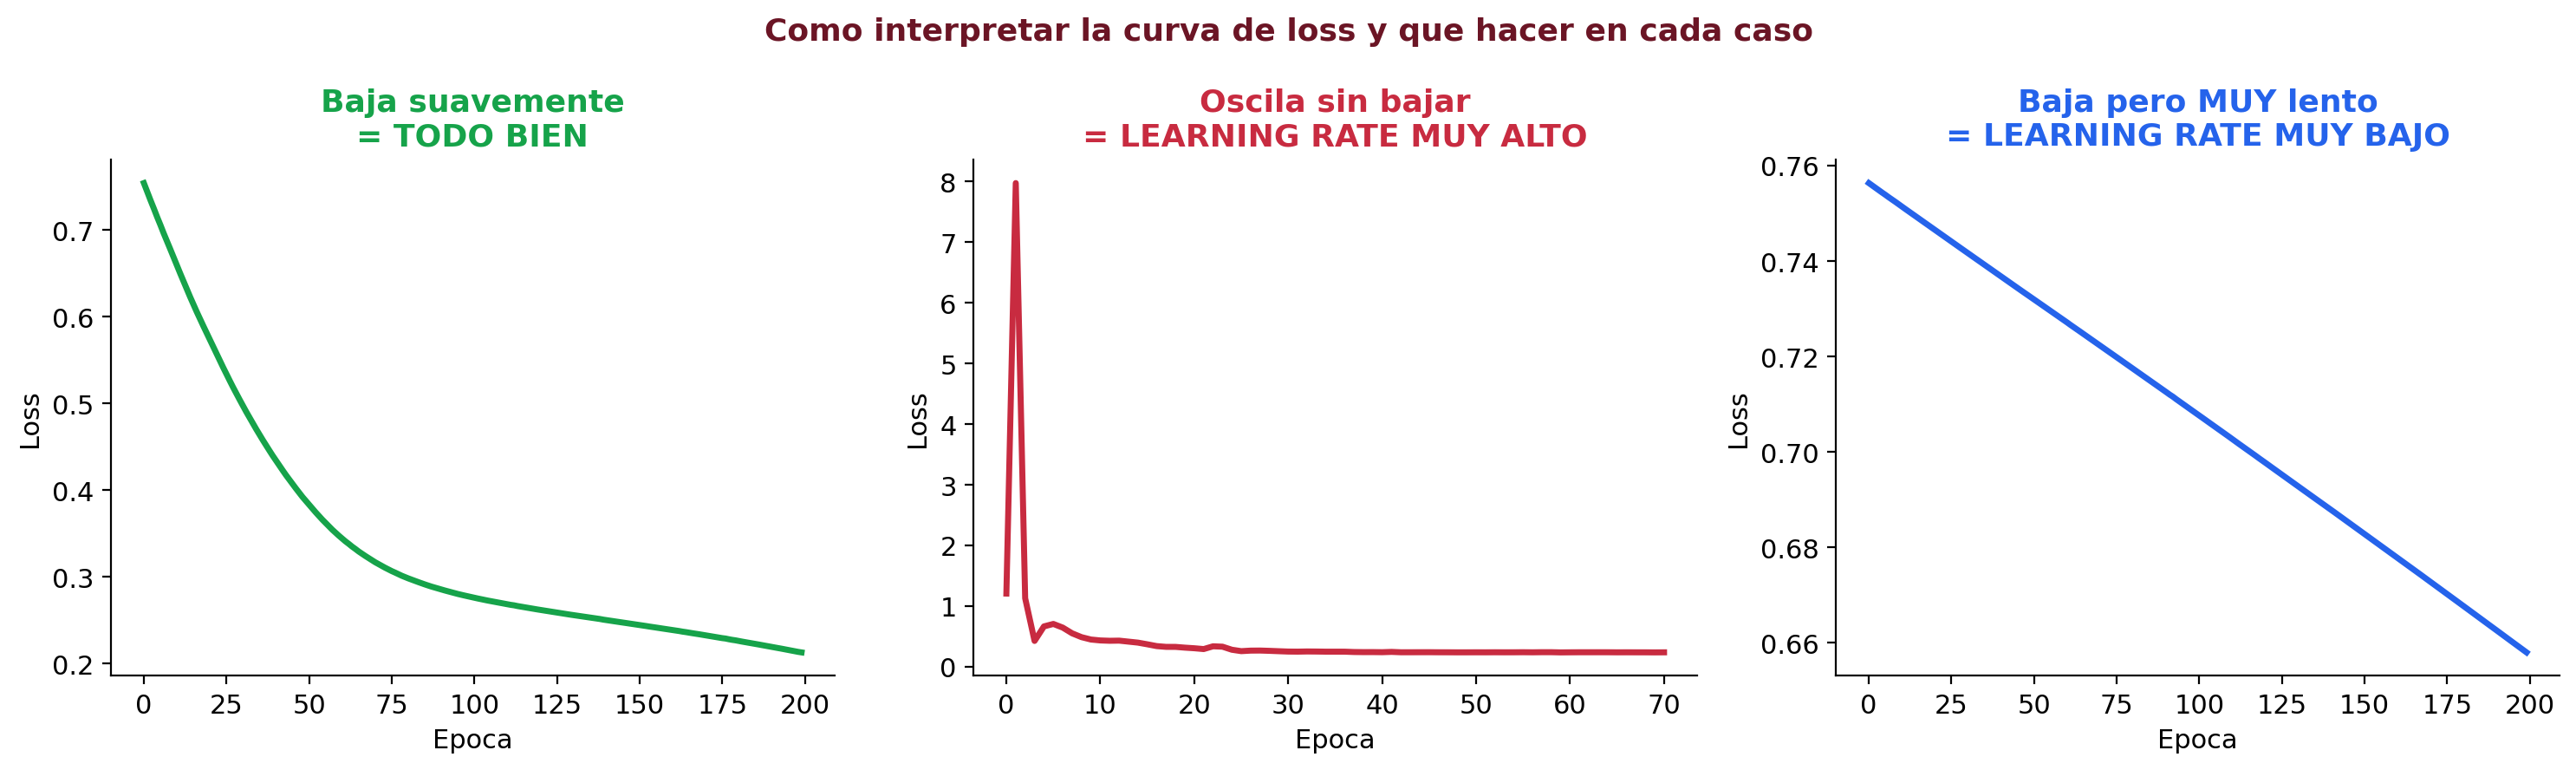
\includegraphics[width=0.95\textwidth]{fig_loss_interpretar.png}
  \end{center}

  \vspace{-2pt}
  {\scriptsize\color{textMuted}
    \faLightbulb\hspace{4pt} \textbf{Izquierda (verde):} baja suavemente
    y se estabiliza --- \textbf{todo bien.}
    \textbf{Centro (rojo):} oscila sin bajar --- \textbf{learning rate
    muy alto}, bajarlo.
    \textbf{Derecha (azul):} baja pero lent\'isimo --- \textbf{learning
    rate muy bajo}, subirlo o m\'as \'epocas.}
\end{frame}

\begin{frame}[shrink=18]{Overfitting en Redes Neuronales}
  \vspace{-4pt}
  \begin{center}
    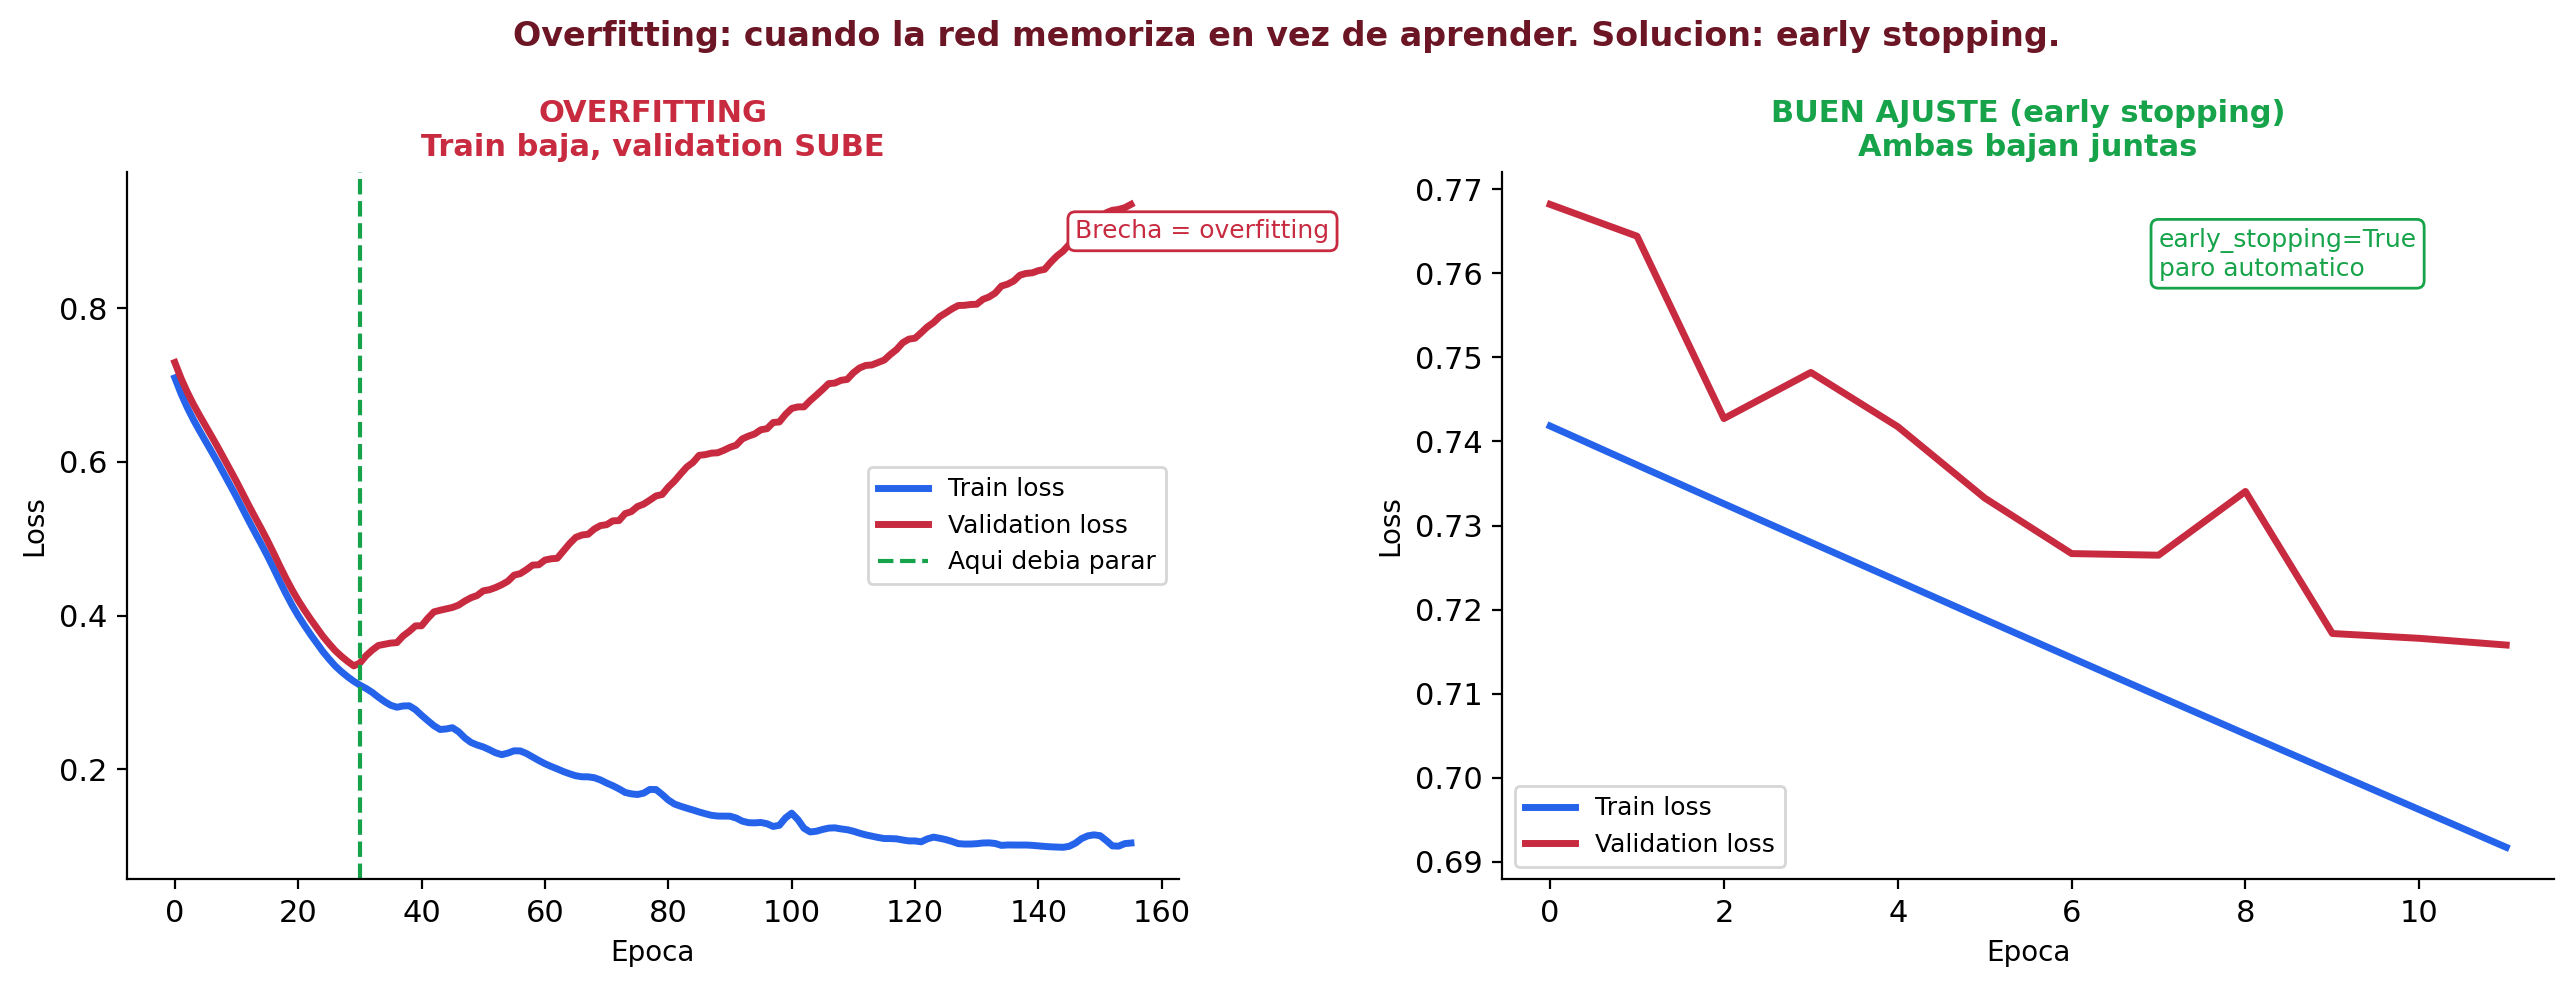
\includegraphics[width=0.88\textwidth]{fig_overfitting_nn.png}
  \end{center}

  \vspace{-2pt}
  {\scriptsize\color{textMuted}
    \faLightbulb\hspace{4pt} \textbf{Izquierda (overfitting):} el loss de
    train baja pero el de validaci\'on \textbf{sube}. La red est\'a
    memorizando. Debi\'o parar en la l\'inea verde.
    \textbf{Derecha (buen ajuste):} con \texttt{early\_stopping=True},
    la red para autom\'aticamente cuando validaci\'on deja de mejorar.
    \textbf{Siempre activar early stopping.}}
\end{frame}

% =============================================================================
%  BLOQUE 5: MLPCLASSIFIER PASO A PASO
% =============================================================================
\sectionframe{MLPClassifier en sklearn}{Import, par\'ametros, c\'odigo completo}

\begin{frame}[fragile,shrink=10]{Paso 1: Importar y Crear el Modelo}
  \vspace{-4pt}
  {\footnotesize\color{arcaDark}\bfseries
    MLPClassifier vive en \texttt{sklearn.neural\_network}:}

  \vspace{4pt}
  \begin{pyblock}
from sklearn.neural_network import MLPClassifier

mlp = MLPClassifier(
    hidden_layer_sizes=(64, 32),   # 2 capas ocultas: 64 y 32 neuronas
    activation="relu",             # ReLU en capas ocultas
    max_iter=300,                  # maximo de epocas
    learning_rate_init=0.001,      # tamano del paso
    early_stopping=True,           # para si no mejora en validacion
    random_state=42)
  \end{pyblock}

  \vspace{4pt}
  {\scriptsize\color{arcaDark}
    \faKey\hspace{4pt} \textbf{Misma API} que log\'istica y RF:
    \texttt{.fit()}, \texttt{.predict()}, \texttt{.predict\_proba()},
    \texttt{.score()}. Cambiar de modelo = cambiar 1 l\'inea.}
\end{frame}

\begin{frame}{Los Par\'ametros Principales}
  \vspace{-4pt}
  {\footnotesize\color{arcaDark}\bfseries
    Los par\'ametros que m\'as van a usar y cu\'ando ajustarlos:}

  \vspace{6pt}
  {\scriptsize
  \begin{tabular}{@{}p{3.8cm}p{2.5cm}p{6cm}@{}}
    \toprule
    \textbf{Par\'ametro} & \textbf{Default} & \textbf{Qu\'e controla} \\
    \midrule
    \texttt{hidden\_layer\_sizes} & \texttt{(100,)} & La arquitectura: cu\'antas capas y neuronas. \texttt{(64, 32)} = 2 capas de 64 y 32 neuronas. \\
    \texttt{activation} & \texttt{"relu"} & Funci\'on de activaci\'on en capas ocultas. ReLU funciona bien en la gran mayor\'ia de casos. \\
    \texttt{max\_iter} & 200 & \'Epocas m\'aximas. Si la red no converge (da warning), se puede subir. \\
    \texttt{learning\_rate\_init} & 0.001 & Tama\~no del paso. Si la curva de loss oscila, bajarlo. Si es muy lenta, subirlo. \\
    \texttt{early\_stopping} & \texttt{False} & Si es \texttt{True}, para autom\'aticamente cuando el error en validaci\'on deja de mejorar. \'Util para prevenir overfitting. \\
    \texttt{alpha} & 0.0001 & Regularizaci\'on L2 --- penaliza pesos grandes (mismo concepto que el C de log\'istica). \\
    \bottomrule
  \end{tabular}
  }

  \vspace{6pt}
  {\scriptsize\color{textMuted}
    \faLightbulb\hspace{4pt} Empezar con los defaults. Despu\'es de entrenar,
    graficar la curva de loss y ajustar seg\'un lo que vean.}
\end{frame}

\begin{frame}[fragile,shrink=18]{Paso 2: Entrenar y Evaluar}
  \vspace{-6pt}
  \begin{pyblock}
from sklearn.model_selection import train_test_split
from sklearn.preprocessing import StandardScaler

# Escalar es IMPORTANTE para redes neuronales
scaler = StandardScaler()
X_train_s = scaler.fit_transform(X_train)
X_test_s = scaler.transform(X_test)

# Entrenar
mlp.fit(X_train_s, y_train)

# Evaluar
print(f"Accuracy train: {mlp.score(X_train_s, y_train):.3f}")
print(f"Accuracy test:  {mlp.score(X_test_s, y_test):.3f}")
print(f"Epocas usadas:  {mlp.n_iter_}")
  \end{pyblock}

  \vspace{4pt}
  {\scriptsize\color{arcaDark}
    \faExclamationTriangle\hspace{4pt} \textbf{StandardScaler es obligatorio}
    para redes neuronales (igual que K-Means). Los pesos iniciales son
    peque\~nos --- si los inputs van de 0 a 255 (pixeles), el gradiente
    explota. Siempre escalar.}
\end{frame}

\begin{frame}[fragile,shrink=10]{Paso 3: Graficar la Curva de Loss}
  \vspace{-4pt}
  {\footnotesize\color{arcaDark}\bfseries
    Siempre despu\'es de entrenar, verificar que convergi\'o:}

  \vspace{4pt}
  \begin{pyblock}
import plotly.express as px

fig = px.line(y=mlp.loss_curve_,
    title="Curva de Loss del MLP",
    labels={"index": "Epoca", "value": "Loss"})
fig.update_layout(template="plotly_white")
fig.show()
  \end{pyblock}

  \vspace{4pt}
  {\scriptsize\color{arcaDark}
  \begin{itemize}\setlength{\itemsep}{3pt}
    \item[{\color{codeGreen}\scriptsize\faCheckCircle}]
      \textbf{Baja suavemente:} todo bien.
    \item[{\color{arcaRed}\scriptsize\faTimesCircle}]
      \textbf{Oscila:} bajar \texttt{learning\_rate\_init}.
    \item[{\color{codeBlue}\scriptsize\faArrowRight}]
      \textbf{Baja muy lento:} subir LR o m\'as \texttt{max\_iter}.
    \item[{\color{codeOrange}\scriptsize\faArrowRight}]
      \textbf{Warning ``no converge'':} subir \texttt{max\_iter} a 500 o 1000.
  \end{itemize}
  }
\end{frame}

\begin{frame}[fragile,shrink=18]{Paso 4: Aplicar a MNIST --- Comparar con RF}
  \vspace{-6pt}
  {\footnotesize\color{arcaDark}\bfseries
    El mismo dataset de la clase 22. ?`Mejora el 95\% de RF?}

  \vspace{4pt}
  \begin{pyblock}
from sklearn.datasets import fetch_openml
import numpy as np

X, y = fetch_openml("mnist_784", version=1,
                     return_X_y=True, as_frame=False, parser="auto")
rng = np.random.default_rng(42)
idx = rng.choice(len(X), 15000, replace=False)
X, y = X[idx], y[idx]

X_train, X_test, y_train, y_test = train_test_split(
    X, y, test_size=0.2, random_state=42)

# Normalizar pixeles
X_train_n, X_test_n = X_train / 255.0, X_test / 255.0

mlp_mnist = MLPClassifier(hidden_layer_sizes=(128, 64),
    max_iter=50, early_stopping=True, random_state=42)
mlp_mnist.fit(X_train_n, y_train)
print(f"MLP Accuracy: {mlp_mnist.score(X_test_n, y_test):.1%}")
  \end{pyblock}
\end{frame}

\begin{frame}{Comparaci\'on: Log\'istica vs RF vs MLP en MNIST}
  \vspace{-4pt}
  {\footnotesize\color{arcaDark}\bfseries
    Los tres modelos en el mismo dataset, las mismas m\'etricas:}

  \vspace{8pt}
  {\footnotesize
  \begin{tabular}{@{}lccl@{}}
    \toprule
    \textbf{Modelo} & \textbf{Accuracy} & \textbf{Tiempo} & \textbf{Tipo de frontera} \\
    \midrule
    Log\'istica & $\approx$ 90\% & R\'apido & L\'inea recta (hiperplano) \\
    Random Forest (200 \'arboles) & $\approx$ 95\% & Medio & Cortes rectangulares \\
    \textbf{MLP (128, 64)} & $\approx$ \textbf{97\%} & Lento & \textbf{Curva suave} \\
    \bottomrule
  \end{tabular}
  }

  \vspace{6pt}
  {\footnotesize
  \begin{itemize}\setlength{\itemsep}{4pt}
    \item[{\color{codeGreen}\scriptsize\faArrowRight}]
      MLP gana en accuracy, especialmente en d\'igitos dif\'iciles
      (3$\leftrightarrow$8, 9$\leftrightarrow$4).
    \item[{\color{arcaRed}\scriptsize\faArrowRight}]
      Pero tarda m\'as en entrenar y tiene m\'as hiperpar\'ametros.
    \item[{\color{arcaRed}\scriptsize\faArrowRight}]
      Y es una \textbf{caja negra}: no podemos inspeccionar
      ``qu\'e pixeles importan'' tan f\'acilmente como en RF.
  \end{itemize}
  }
\end{frame}

\begin{frame}[shrink=18]{MLP Resuelve los 3 Problemas No Lineales}
  \vspace{-4pt}
  \begin{center}
    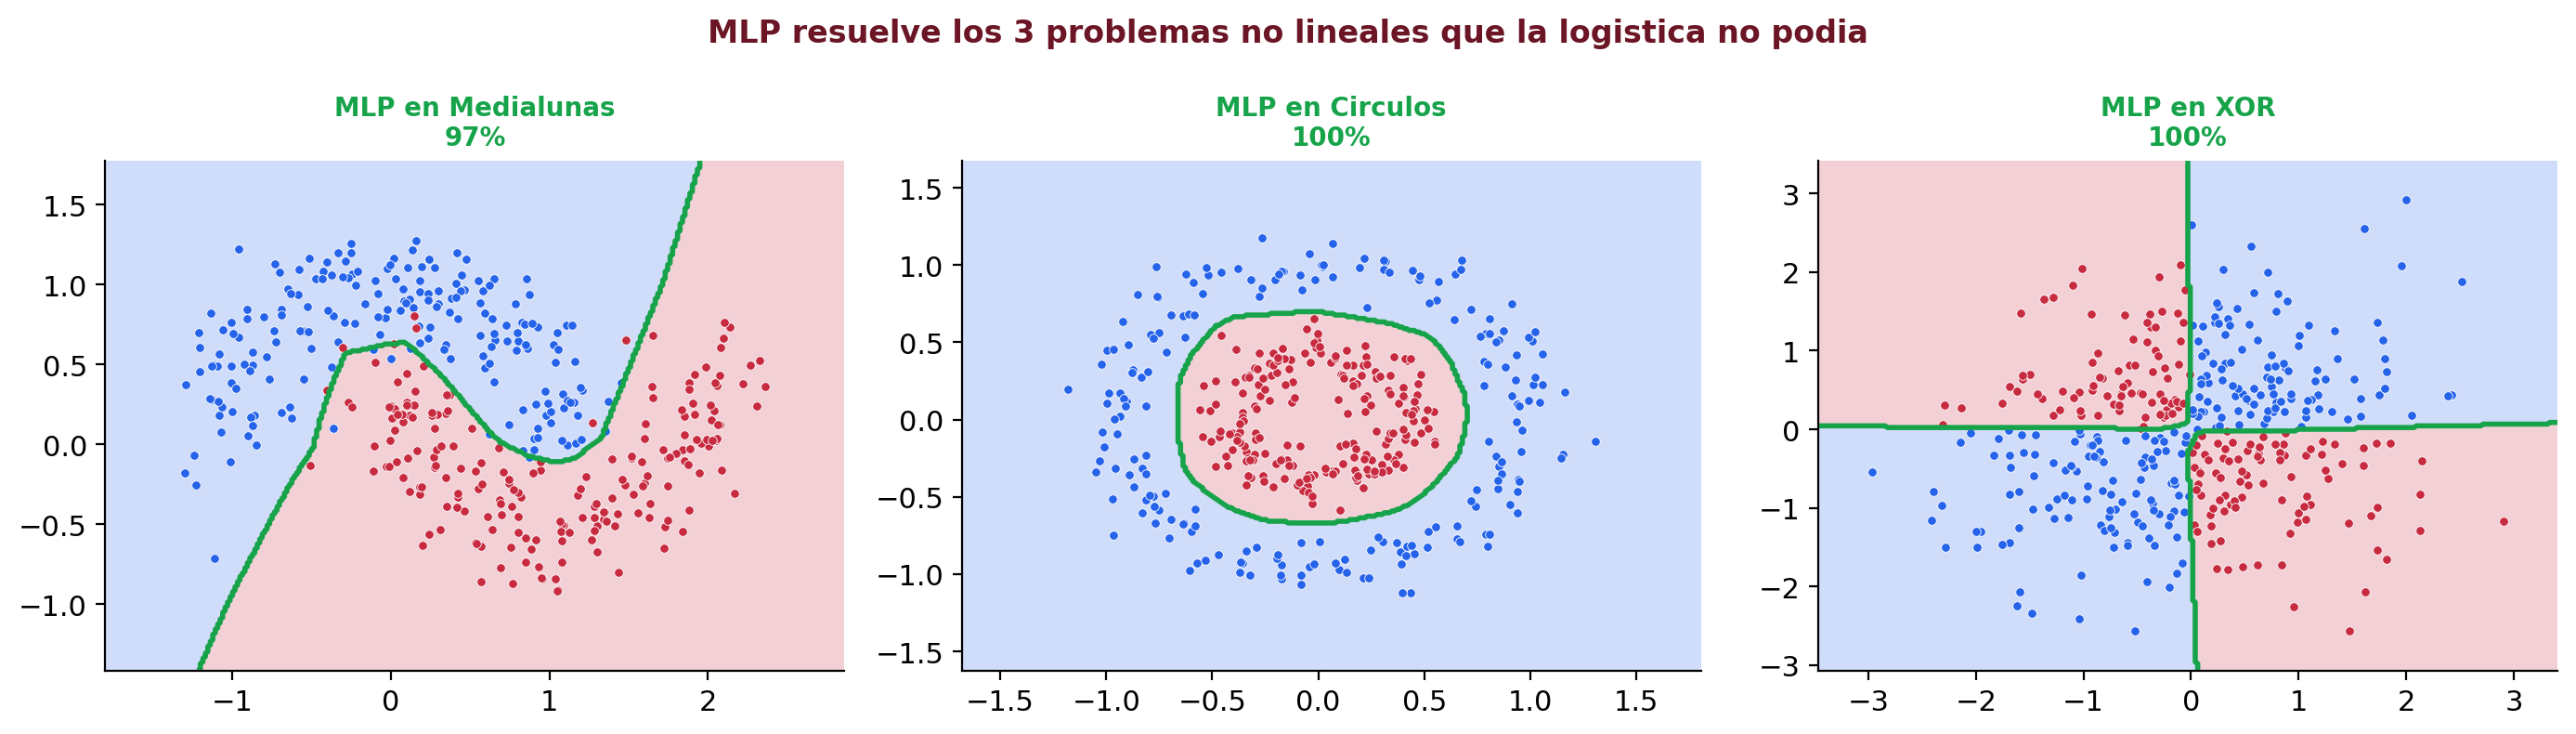
\includegraphics[width=0.88\textwidth]{fig_mlp_resuelve.png}
  \end{center}

  \vspace{-2pt}
  {\scriptsize\color{textMuted}
    \faLightbulb\hspace{4pt} \textbf{Medialunas:} curva suave que las separa
    (100\%). \textbf{C\'irculos:} frontera circular (100\%).
    \textbf{XOR:} 4 regiones alternadas (99\%).
    La misma arquitectura (32, 16) + ReLU resuelve los 3 problemas
    que la log\'istica no pod\'ia.}
\end{frame}

\begin{frame}[shrink=5]{Ejercicio 2: MLP en MNIST}
  \vspace{-4pt}
  {\footnotesize\color{arcaDark}\bfseries
    \faClock\hspace{4pt} 10 minutos --- en el notebook:}

  \vspace{6pt}
  {\footnotesize
  \begin{enumerate}\setlength{\itemsep}{4pt}
    \item[{\color{arcaRed}\bfseries 1.}]
      Copien el c\'odigo del slide anterior para cargar MNIST.
    \item[{\color{arcaRed}\bfseries 2.}]
      Entrenen un MLP con \texttt{(128, 64)}, \texttt{max\_iter=50},
      \texttt{early\_stopping=True}.
    \item[{\color{arcaRed}\bfseries 3.}]
      Grafiquen la curva de loss. ?`Convergi\'o?
    \item[{\color{arcaRed}\bfseries 4.}]
      Generen la confusion matrix (\texttt{ConfusionMatrixDisplay}).
      ?`Qu\'e d\'igitos sigue confundiendo?
    \item[{\color{codeGreen}\bfseries 5.}]
      Comparen el accuracy con la log\'istica y RF de la clase 22.
    \item[{\color{codeGreen}\bfseries 6.}]
      \textbf{Bonus:} prueben \texttt{(256, 128, 64)}. ?`Mejora?
      ?`Tarda m\'as?
  \end{enumerate}
  }
\end{frame}

% =============================================================================
%  BLOQUE 6: CRITERIOS DE DISE\~NO Y CU\'ANDO USAR NN
% =============================================================================
\sectionframe{Criterios de Dise\~no}{Cu\'antas capas, cu\'antas neuronas, cu\'ando usar NN}

\begin{frame}{?`Cu\'antas Capas y Cu\'antas Neuronas?}
  \vspace{-4pt}
  {\footnotesize\color{arcaDark}\bfseries
    No hay f\'ormula m\'agica, pero hay gu\'ias pr\'acticas:}

  \vspace{6pt}
  {\scriptsize
  \begin{tabular}{@{}p{3cm}p{3cm}p{2.5cm}p{3.5cm}@{}}
    \toprule
    \textbf{Problema} & \textbf{Arquitectura} & \textbf{Ejemplo} & \textbf{Raz\'on} \\
    \midrule
    Tabular simple (pocos features) & 1 capa, 32--64 neuronas & \texttt{(64,)} & Pocas variables, relaciones simples. \\
    Tabular complejo (muchos features) & 2 capas, piramidal & \texttt{(128, 64)} & M\'as features = m\'as patrones que combinar. \\
    Im\'agenes peque\~nas (MNIST) & 2 capas, 128--256 & \texttt{(256, 128)} & 784 inputs necesitan m\'as neuronas para comprimir. \\
    Im\'agenes reales & CNN (no MLP) & --- & MLP no captura estructura espacial. \\
    \bottomrule
  \end{tabular}
  }

  \vspace{6pt}
  {\footnotesize
  \begin{itemize}\setlength{\itemsep}{3pt}
    \item[{\color{codeGreen}\scriptsize\faArrowRight}]
      \textbf{Forma piramidal:} cada capa tiene menos neuronas que la anterior
      (128 $\to$ 64 $\to$ 32). Comprime la informaci\'on gradualmente.
    \item[{\color{arcaRed}\scriptsize\faArrowRight}]
      \textbf{Empezar peque\~no:} \texttt{(64, 32)} primero. Si no
      funciona, agrandar. M\'as f\'acil hacer crecer que recortar.
  \end{itemize}
  }
\end{frame}

\begin{frame}{Criterios para Elegir la Arquitectura}
  \vspace{-4pt}
  {\footnotesize\color{arcaDark}\bfseries
    Orden de decisiones:}

  \vspace{6pt}
  {\footnotesize
  \begin{enumerate}\setlength{\itemsep}{5pt}
    \item[{\color{arcaRed}\bfseries 1.}]
      \textbf{?`Cu\'antas capas?} Empezar con 1--2. Agregar una tercera
      solo si 2 capas no alcanzan. M\'as de 3 rara vez ayuda en sklearn.
    \item[{\color{arcaRed}\bfseries 2.}]
      \textbf{?`Cu\'antas neuronas?} Primera capa: entre la cantidad
      de features y 2$\times$ features. Siguientes capas: reducir
      a la mitad. Nunca menos que el n\'umero de clases.
    \item[{\color{arcaRed}\bfseries 3.}]
      \textbf{Entrenar y ver la curva de loss.} Si no converge,
      m\'as \'epocas o ajustar LR. Si hay overfitting, reducir
      o activar early stopping.
    \item[{\color{codeGreen}\bfseries 4.}]
      \textbf{Comparar con el modelo anterior.} Si MLP no mejora
      significativamente sobre RF, usar RF (m\'as simple, m\'as
      interpretable).
  \end{enumerate}
  }

  \vspace{4pt}
  \begin{tcolorbox}[colback=arcaGray, colframe=arcaRed, boxrule=0.5pt, arc=2pt,
    left=6pt, right=6pt, top=4pt, bottom=4pt]
    {\scriptsize\color{arcaDark}
    \faKey\hspace{4pt}\textbf{El mejor modelo no es el m\'as complejo.}
    Es el que resuelve el problema con la complejidad justa.}
  \end{tcolorbox}
\end{frame}

\begin{frame}{?`Cu\'ando Usar Cada Modelo?}
  \vspace{-4pt}
  {\scriptsize
  \begin{tabular}{@{}p{2.5cm}p{3cm}p{3cm}p{3.5cm}@{}}
    \toprule
     & \textbf{\color{codeBlue}Log\'istica} & \textbf{\color{codeOrange}Random Forest} & \textbf{\color{arcaRed}Red Neuronal (MLP)} \\
    \midrule
    \textbf{Frontera} & L\'inea recta & Rectangular (cortes) & Curva suave \\
    \textbf{Interpretable} & S\'i (coeficientes) & Parcial (importancia) & No (caja negra) \\
    \textbf{Velocidad} & Muy r\'apido & R\'apido & Lento \\
    \textbf{Datos necesarios} & Pocos ($<$ 1K) & Medio (1K--10K) & Muchos ($>$ 5K) \\
    \textbf{Hiperpar\'ametros} & 1--2 & 3--4 & 5+ \\
    \textbf{Escalar} & S\'i & No necesita & \textbf{Obligatorio} \\
    \textbf{Mejor para} & Baseline siempre & Datos tabulares & Im\'agenes, mucho dato \\
    \bottomrule
  \end{tabular}
  }

  \vspace{6pt}
  \begin{tcolorbox}[colback=codeGreen!8, colframe=codeGreen, boxrule=0.5pt, arc=2pt,
    left=6pt, right=6pt, top=4pt, bottom=4pt]
    {\scriptsize\color{arcaDark}
    \faLightbulb\hspace{4pt}\textbf{Flujo recomendado:}
    siempre empezar con log\'istica (baseline) $\to$ RF
    (si la log\'istica no alcanza) $\to$ MLP (solo si RF
    tampoco alcanza o si los datos son im\'agenes).
    Nunca saltar directamente a redes neuronales.}
  \end{tcolorbox}
\end{frame}

\begin{frame}{?`Por Qu\'e No Usar Siempre Redes Neuronales?}
  \vspace{-4pt}
  {\footnotesize\color{arcaDark}\bfseries
    Si las redes neuronales son tan poderosas, ?`por qu\'e no usarlas
    para todo?}

  \vspace{6pt}
  {\footnotesize
  \begin{itemize}\setlength{\itemsep}{5pt}
    \item[{\color{arcaRed}\scriptsize\faTimesCircle}]
      \textbf{Pocos datos:} con 200 filas, una NN memoriza todo
      (overfitting). RF funciona mejor con pocos datos.
    \item[{\color{arcaRed}\scriptsize\faTimesCircle}]
      \textbf{Interpretabilidad:} un gerente quiere saber \textit{por qu\'e}
      el modelo predijo algo. En log\'istica puedes decir ``la glucosa
      alta subi\'o la probabilidad''. En una NN no puedes.
    \item[{\color{arcaRed}\scriptsize\faTimesCircle}]
      \textbf{Tiempo:} RF entrena en segundos, MLP en minutos u horas.
      Si el resultado es similar, RF gana.
    \item[{\color{arcaRed}\scriptsize\faTimesCircle}]
      \textbf{Complejidad:} m\'as hiperpar\'ametros = m\'as cosas que
      pueden salir mal (LR, capas, \'epocas, batch size, regularizaci\'on).
  \end{itemize}
  }

  \vspace{4pt}
  {\scriptsize\color{textMuted}
    \faLightbulb\hspace{4pt} En la industria, la mayor\'ia de problemas
    tabulares se resuelven con gradient boosting (XGBoost, LightGBM)
    o Random Forest. Las redes neuronales dominan en im\'agenes,
    texto y audio.}
\end{frame}

\begin{frame}{Las Limitaciones del MLP: ?`Qu\'e No Puede Hacer?}
  \vspace{-4pt}
  {\footnotesize\color{arcaDark}\bfseries
    El MLP es poderoso, pero tiene l\'imites fundamentales
    cuando trabaja con im\'agenes:}

  \vspace{6pt}
  {\footnotesize
  \begin{itemize}\setlength{\itemsep}{5pt}
    \item[{\color{arcaRed}\scriptsize\faTimesCircle}]
      \textbf{Aplana la imagen:} convierte 28$\times$28 en un vector
      de 784 n\'umeros. \textbf{Pierde la estructura espacial} ---
      no sabe que el pixel 100 est\'a \textit{al lado} del pixel 101.
    \item[{\color{arcaRed}\scriptsize\faTimesCircle}]
      \textbf{No es invariante a posici\'on:} un ``3'' centrado y un
      ``3'' desplazado 5 pixeles son vectores \textbf{completamente
      distintos} para el MLP. Tiene que aprender cada posici\'on
      por separado.
    \item[{\color{arcaRed}\scriptsize\faTimesCircle}]
      \textbf{Demasiados par\'ametros:} 784 inputs $\times$ 128
      neuronas = 100\,000 pesos solo en la primera capa. F\'acil
      de sobreajustar y lento de entrenar.
    \item[{\color{arcaRed}\scriptsize\faTimesCircle}]
      \textbf{No escala a im\'agenes reales:} una foto de
      224$\times$224$\times$3 = 150\,000 inputs. El MLP
      necesitar\'ia millones de pesos.
  \end{itemize}
  }
\end{frame}

\begin{frame}{?`Qu\'e Viene Despu\'es? --- Redes Convolucionales (CNN)}
  \vspace{-4pt}
  {\footnotesize\color{arcaDark}\bfseries
    Las CNNs resuelven exactamente los problemas del MLP:}

  \vspace{6pt}
  {\footnotesize
  \begin{itemize}\setlength{\itemsep}{5pt}
    \item[{\color{codeGreen}\scriptsize\faCheckCircle}]
      \textbf{Procesan la imagen como imagen} (2D), no como vector.
      Mantienen la estructura espacial.
    \item[{\color{codeGreen}\scriptsize\faCheckCircle}]
      \textbf{Filtros locales:} en vez de conectar cada pixel con cada
      neurona, usan ventanas peque\~nas (3$\times$3) que recorren la
      imagen detectando bordes, curvas, texturas.
    \item[{\color{codeGreen}\scriptsize\faCheckCircle}]
      \textbf{Invariancia a posici\'on:} el mismo filtro se aplica en
      toda la imagen. Un ``3'' se detecta sin importar d\'onde est\'e.
    \item[{\color{codeGreen}\scriptsize\faCheckCircle}]
      \textbf{Muchos menos par\'ametros:} un filtro 3$\times$3 tiene
      9 pesos, no 100\,000.
  \end{itemize}
  }

  \vspace{4pt}
  \begin{tcolorbox}[colback=codeGreen!8, colframe=codeGreen, boxrule=0.5pt, arc=2pt,
    left=6pt, right=6pt, top=4pt, bottom=4pt]
    {\scriptsize\color{arcaDark}
    \faArrowRight\hspace{4pt}\textbf{Pr\'oximas clases:} construiremos
    CNNs paso a paso. Todo lo que aprendieron hoy (pesos, activaciones,
    backprop, curva de loss, early stopping) se reutiliza. Solo cambia
    la \textbf{arquitectura} --- de fully connected a convolucional.}
  \end{tcolorbox}
\end{frame}

% =============================================================================
%  CIERRE
% =============================================================================
\sectionframe{Cierre}{Lo que aprendimos hoy}

\begin{frame}[shrink=10]{Resumen}
  \vspace{-4pt}
  \begin{columns}[T]
    \begin{column}{0.48\textwidth}
      {\footnotesize\bfseries\color{arcaDark} De log\'istica a neurona:}
      \vspace{3pt}
      {\footnotesize
      \begin{itemize}\setlength{\itemsep}{2pt}
        \item[{\color{codeGreen}\faCheckCircle}]
          Log\'istica = 1 neurona con sigmoid.
        \item[{\color{codeGreen}\faCheckCircle}]
          Pesos $w$ = coeficientes $\beta$.
        \item[{\color{codeGreen}\faCheckCircle}]
          1 neurona = 1 l\'inea recta. No basta.
        \item[{\color{codeGreen}\faCheckCircle}]
          ReLU en ocultas, sigmoid/softmax en salida.
      \end{itemize}
      }
      \vspace{3pt}
      {\footnotesize\bfseries\color{codeBlue} Conectar neuronas:}
      \vspace{3pt}
      {\footnotesize
      \begin{itemize}\setlength{\itemsep}{2pt}
        \item[{\color{codeGreen}\faCheckCircle}]
          Cada conexi\'on: un n\'umero $\times$ un peso.
        \item[{\color{codeGreen}\faCheckCircle}]
          M\'as capas = fronteras m\'as complejas.
        \item[{\color{codeGreen}\faCheckCircle}]
          Cada capa detecta patrones m\'as abstractos.
      \end{itemize}
      }
    \end{column}
    \begin{column}{0.48\textwidth}
      {\footnotesize\bfseries\color{arcaRed} C\'omo aprende:}
      \vspace{3pt}
      {\footnotesize
      \begin{itemize}\setlength{\itemsep}{2pt}
        \item[{\color{codeGreen}\faCheckCircle}]
          Forward $\to$ loss $\to$ backprop $\to$ update.
        \item[{\color{codeGreen}\faCheckCircle}]
          Siempre graficar la curva de loss.
        \item[{\color{codeGreen}\faCheckCircle}]
          Siempre \texttt{early\_stopping=True}.
      \end{itemize}
      }
      \vspace{3pt}
      {\footnotesize\bfseries\color{codePurple} MLPClassifier:}
      \vspace{3pt}
      {\footnotesize
      \begin{itemize}\setlength{\itemsep}{2pt}
        \item[{\color{codeGreen}\faCheckCircle}]
          Misma API de sklearn (\texttt{.fit}, \texttt{.predict}).
        \item[{\color{codeGreen}\faCheckCircle}]
          \texttt{hidden\_layer\_sizes}: forma piramidal.
        \item[{\color{codeGreen}\faCheckCircle}]
          StandardScaler obligatorio.
        \item[{\color{codeGreen}\faCheckCircle}]
          Usar NN solo cuando RF no alcanza.
      \end{itemize}
      }
    \end{column}
  \end{columns}
\end{frame}

% ── QR ENCUESTA ──────────────────────────────────────────────────────────────
{
\setbeamertemplate{headline}{}
\setbeamertemplate{footline}{}
\begin{frame}[plain, noframenumbering]
  \begin{tikzpicture}[remember picture, overlay]
    \fill[arcaDark] (current page.south west) rectangle (current page.north east);
  \end{tikzpicture}
  \vspace{1cm}
  \begin{center}
    {\Huge\bfseries\color{white} ?`C\'omo estuvo la clase?\par}
    \vspace{0.6cm}
    
\includegraphics[width=4cm]{qr_encuesta.jpg}
    \vspace{0.4cm}

    {\large\color{white!80} Escanea el QR para dejarnos tu opini\'on.\par}
  \end{center}
\end{frame}
}

\end{document}
